% Generated by Sphinx.
\def\sphinxdocclass{report}
\documentclass[letterpaper,10pt,french]{sphinxmanual}
\usepackage[utf8]{inputenc}
\DeclareUnicodeCharacter{00A0}{\nobreakspace}
\usepackage{cmap}
\usepackage[T1]{fontenc}
\usepackage{babel}
\usepackage{times}
\usepackage[Sonny]{fncychap}
\usepackage{longtable}
\usepackage{sphinx}
\usepackage{multirow}


\title{Conception et développement   d’une version du site adaptée à l’utilisation sur smartphone ou tablette}
\date{14 January 2015}
\release{0.1}
\author{Daniel Filipe Nunes Silva}
\newcommand{\sphinxlogo}{}
\renewcommand{\releasename}{Version}
\makeindex

\makeatletter
\def\PYG@reset{\let\PYG@it=\relax \let\PYG@bf=\relax%
    \let\PYG@ul=\relax \let\PYG@tc=\relax%
    \let\PYG@bc=\relax \let\PYG@ff=\relax}
\def\PYG@tok#1{\csname PYG@tok@#1\endcsname}
\def\PYG@toks#1+{\ifx\relax#1\empty\else%
    \PYG@tok{#1}\expandafter\PYG@toks\fi}
\def\PYG@do#1{\PYG@bc{\PYG@tc{\PYG@ul{%
    \PYG@it{\PYG@bf{\PYG@ff{#1}}}}}}}
\def\PYG#1#2{\PYG@reset\PYG@toks#1+\relax+\PYG@do{#2}}

\expandafter\def\csname PYG@tok@c\endcsname{\let\PYG@it=\textit\def\PYG@tc##1{\textcolor[rgb]{0.25,0.50,0.56}{##1}}}
\expandafter\def\csname PYG@tok@il\endcsname{\def\PYG@tc##1{\textcolor[rgb]{0.13,0.50,0.31}{##1}}}
\expandafter\def\csname PYG@tok@gs\endcsname{\let\PYG@bf=\textbf}
\expandafter\def\csname PYG@tok@k\endcsname{\let\PYG@bf=\textbf\def\PYG@tc##1{\textcolor[rgb]{0.00,0.44,0.13}{##1}}}
\expandafter\def\csname PYG@tok@ow\endcsname{\let\PYG@bf=\textbf\def\PYG@tc##1{\textcolor[rgb]{0.00,0.44,0.13}{##1}}}
\expandafter\def\csname PYG@tok@kr\endcsname{\let\PYG@bf=\textbf\def\PYG@tc##1{\textcolor[rgb]{0.00,0.44,0.13}{##1}}}
\expandafter\def\csname PYG@tok@s1\endcsname{\def\PYG@tc##1{\textcolor[rgb]{0.25,0.44,0.63}{##1}}}
\expandafter\def\csname PYG@tok@cm\endcsname{\let\PYG@it=\textit\def\PYG@tc##1{\textcolor[rgb]{0.25,0.50,0.56}{##1}}}
\expandafter\def\csname PYG@tok@gi\endcsname{\def\PYG@tc##1{\textcolor[rgb]{0.00,0.63,0.00}{##1}}}
\expandafter\def\csname PYG@tok@vg\endcsname{\def\PYG@tc##1{\textcolor[rgb]{0.73,0.38,0.84}{##1}}}
\expandafter\def\csname PYG@tok@gp\endcsname{\let\PYG@bf=\textbf\def\PYG@tc##1{\textcolor[rgb]{0.78,0.36,0.04}{##1}}}
\expandafter\def\csname PYG@tok@sr\endcsname{\def\PYG@tc##1{\textcolor[rgb]{0.14,0.33,0.53}{##1}}}
\expandafter\def\csname PYG@tok@s\endcsname{\def\PYG@tc##1{\textcolor[rgb]{0.25,0.44,0.63}{##1}}}
\expandafter\def\csname PYG@tok@si\endcsname{\let\PYG@it=\textit\def\PYG@tc##1{\textcolor[rgb]{0.44,0.63,0.82}{##1}}}
\expandafter\def\csname PYG@tok@ge\endcsname{\let\PYG@it=\textit}
\expandafter\def\csname PYG@tok@nn\endcsname{\let\PYG@bf=\textbf\def\PYG@tc##1{\textcolor[rgb]{0.05,0.52,0.71}{##1}}}
\expandafter\def\csname PYG@tok@kd\endcsname{\let\PYG@bf=\textbf\def\PYG@tc##1{\textcolor[rgb]{0.00,0.44,0.13}{##1}}}
\expandafter\def\csname PYG@tok@cp\endcsname{\def\PYG@tc##1{\textcolor[rgb]{0.00,0.44,0.13}{##1}}}
\expandafter\def\csname PYG@tok@nd\endcsname{\let\PYG@bf=\textbf\def\PYG@tc##1{\textcolor[rgb]{0.33,0.33,0.33}{##1}}}
\expandafter\def\csname PYG@tok@m\endcsname{\def\PYG@tc##1{\textcolor[rgb]{0.13,0.50,0.31}{##1}}}
\expandafter\def\csname PYG@tok@sx\endcsname{\def\PYG@tc##1{\textcolor[rgb]{0.78,0.36,0.04}{##1}}}
\expandafter\def\csname PYG@tok@kc\endcsname{\let\PYG@bf=\textbf\def\PYG@tc##1{\textcolor[rgb]{0.00,0.44,0.13}{##1}}}
\expandafter\def\csname PYG@tok@kp\endcsname{\def\PYG@tc##1{\textcolor[rgb]{0.00,0.44,0.13}{##1}}}
\expandafter\def\csname PYG@tok@se\endcsname{\let\PYG@bf=\textbf\def\PYG@tc##1{\textcolor[rgb]{0.25,0.44,0.63}{##1}}}
\expandafter\def\csname PYG@tok@s2\endcsname{\def\PYG@tc##1{\textcolor[rgb]{0.25,0.44,0.63}{##1}}}
\expandafter\def\csname PYG@tok@gr\endcsname{\def\PYG@tc##1{\textcolor[rgb]{1.00,0.00,0.00}{##1}}}
\expandafter\def\csname PYG@tok@kt\endcsname{\def\PYG@tc##1{\textcolor[rgb]{0.56,0.13,0.00}{##1}}}
\expandafter\def\csname PYG@tok@sd\endcsname{\let\PYG@it=\textit\def\PYG@tc##1{\textcolor[rgb]{0.25,0.44,0.63}{##1}}}
\expandafter\def\csname PYG@tok@mb\endcsname{\def\PYG@tc##1{\textcolor[rgb]{0.13,0.50,0.31}{##1}}}
\expandafter\def\csname PYG@tok@sb\endcsname{\def\PYG@tc##1{\textcolor[rgb]{0.25,0.44,0.63}{##1}}}
\expandafter\def\csname PYG@tok@mo\endcsname{\def\PYG@tc##1{\textcolor[rgb]{0.13,0.50,0.31}{##1}}}
\expandafter\def\csname PYG@tok@nl\endcsname{\let\PYG@bf=\textbf\def\PYG@tc##1{\textcolor[rgb]{0.00,0.13,0.44}{##1}}}
\expandafter\def\csname PYG@tok@nt\endcsname{\let\PYG@bf=\textbf\def\PYG@tc##1{\textcolor[rgb]{0.02,0.16,0.45}{##1}}}
\expandafter\def\csname PYG@tok@o\endcsname{\def\PYG@tc##1{\textcolor[rgb]{0.40,0.40,0.40}{##1}}}
\expandafter\def\csname PYG@tok@w\endcsname{\def\PYG@tc##1{\textcolor[rgb]{0.73,0.73,0.73}{##1}}}
\expandafter\def\csname PYG@tok@vi\endcsname{\def\PYG@tc##1{\textcolor[rgb]{0.73,0.38,0.84}{##1}}}
\expandafter\def\csname PYG@tok@cs\endcsname{\def\PYG@tc##1{\textcolor[rgb]{0.25,0.50,0.56}{##1}}\def\PYG@bc##1{\setlength{\fboxsep}{0pt}\colorbox[rgb]{1.00,0.94,0.94}{\strut ##1}}}
\expandafter\def\csname PYG@tok@nb\endcsname{\def\PYG@tc##1{\textcolor[rgb]{0.00,0.44,0.13}{##1}}}
\expandafter\def\csname PYG@tok@nf\endcsname{\def\PYG@tc##1{\textcolor[rgb]{0.02,0.16,0.49}{##1}}}
\expandafter\def\csname PYG@tok@mh\endcsname{\def\PYG@tc##1{\textcolor[rgb]{0.13,0.50,0.31}{##1}}}
\expandafter\def\csname PYG@tok@ne\endcsname{\def\PYG@tc##1{\textcolor[rgb]{0.00,0.44,0.13}{##1}}}
\expandafter\def\csname PYG@tok@gu\endcsname{\let\PYG@bf=\textbf\def\PYG@tc##1{\textcolor[rgb]{0.50,0.00,0.50}{##1}}}
\expandafter\def\csname PYG@tok@nc\endcsname{\let\PYG@bf=\textbf\def\PYG@tc##1{\textcolor[rgb]{0.05,0.52,0.71}{##1}}}
\expandafter\def\csname PYG@tok@sc\endcsname{\def\PYG@tc##1{\textcolor[rgb]{0.25,0.44,0.63}{##1}}}
\expandafter\def\csname PYG@tok@err\endcsname{\def\PYG@bc##1{\setlength{\fboxsep}{0pt}\fcolorbox[rgb]{1.00,0.00,0.00}{1,1,1}{\strut ##1}}}
\expandafter\def\csname PYG@tok@ni\endcsname{\let\PYG@bf=\textbf\def\PYG@tc##1{\textcolor[rgb]{0.84,0.33,0.22}{##1}}}
\expandafter\def\csname PYG@tok@go\endcsname{\def\PYG@tc##1{\textcolor[rgb]{0.20,0.20,0.20}{##1}}}
\expandafter\def\csname PYG@tok@gt\endcsname{\def\PYG@tc##1{\textcolor[rgb]{0.00,0.27,0.87}{##1}}}
\expandafter\def\csname PYG@tok@gd\endcsname{\def\PYG@tc##1{\textcolor[rgb]{0.63,0.00,0.00}{##1}}}
\expandafter\def\csname PYG@tok@gh\endcsname{\let\PYG@bf=\textbf\def\PYG@tc##1{\textcolor[rgb]{0.00,0.00,0.50}{##1}}}
\expandafter\def\csname PYG@tok@mf\endcsname{\def\PYG@tc##1{\textcolor[rgb]{0.13,0.50,0.31}{##1}}}
\expandafter\def\csname PYG@tok@kn\endcsname{\let\PYG@bf=\textbf\def\PYG@tc##1{\textcolor[rgb]{0.00,0.44,0.13}{##1}}}
\expandafter\def\csname PYG@tok@sh\endcsname{\def\PYG@tc##1{\textcolor[rgb]{0.25,0.44,0.63}{##1}}}
\expandafter\def\csname PYG@tok@na\endcsname{\def\PYG@tc##1{\textcolor[rgb]{0.25,0.44,0.63}{##1}}}
\expandafter\def\csname PYG@tok@mi\endcsname{\def\PYG@tc##1{\textcolor[rgb]{0.13,0.50,0.31}{##1}}}
\expandafter\def\csname PYG@tok@bp\endcsname{\def\PYG@tc##1{\textcolor[rgb]{0.00,0.44,0.13}{##1}}}
\expandafter\def\csname PYG@tok@c1\endcsname{\let\PYG@it=\textit\def\PYG@tc##1{\textcolor[rgb]{0.25,0.50,0.56}{##1}}}
\expandafter\def\csname PYG@tok@vc\endcsname{\def\PYG@tc##1{\textcolor[rgb]{0.73,0.38,0.84}{##1}}}
\expandafter\def\csname PYG@tok@nv\endcsname{\def\PYG@tc##1{\textcolor[rgb]{0.73,0.38,0.84}{##1}}}
\expandafter\def\csname PYG@tok@no\endcsname{\def\PYG@tc##1{\textcolor[rgb]{0.38,0.68,0.84}{##1}}}
\expandafter\def\csname PYG@tok@ss\endcsname{\def\PYG@tc##1{\textcolor[rgb]{0.32,0.47,0.09}{##1}}}

\def\PYGZbs{\char`\\}
\def\PYGZus{\char`\_}
\def\PYGZob{\char`\{}
\def\PYGZcb{\char`\}}
\def\PYGZca{\char`\^}
\def\PYGZam{\char`\&}
\def\PYGZlt{\char`\<}
\def\PYGZgt{\char`\>}
\def\PYGZsh{\char`\#}
\def\PYGZpc{\char`\%}
\def\PYGZdl{\char`\$}
\def\PYGZhy{\char`\-}
\def\PYGZsq{\char`\'}
\def\PYGZdq{\char`\"}
\def\PYGZti{\char`\~}
% for compatibility with earlier versions
\def\PYGZat{@}
\def\PYGZlb{[}
\def\PYGZrb{]}
\makeatother

\renewcommand\PYGZsq{\textquotesingle}

\begin{document}

\maketitle
\tableofcontents
\phantomsection\label{index::doc}



\chapter{Introduction}
\label{intro::doc}\label{intro:bienvenue-sur-le-travail-ecrit}\label{intro:introduction}
Notre monde actuel devient chaque année plus proche de la technologie et se veut
devenir petit à petit un monde connecté. Ceci est sans doute une des raisons
pour lesquelles ce séminaire de développement d'une platforme de formation
en ligne a été lancé. En effet, grâce à l'informatique, nous pouvons élaborer
des techniques d'enseignement qui n'étaient pas disponibles il y a quelques
années, ce qui sous-entend que la pédagogie de l'époque n'était pas la même qu'aujourd'hui et que
celle-ci évolue au fil du temps. De ce fait, il nous faut constamment se mettre à jour si l'on
veut explorer d'autres moyens d'étude et d'enseignement. Je vais, dans ce travail,
programmer une application web en version mobile qui permettra aux élèves de
communiquer avec leurs professeurs. Non pas par l'échange de mots mais par le
téléversement d'images. Le but premier de mon travail est de fournir au professeur
un outil grâce auquel il pourra par exemple demander à ses élèves de faire un
exercice et le photographier avec leurs smartphones avant de l'envoyer sur un serveur auquel celui-là
aura accès et pourra donc voir les différentes résolutions du travail de ses élèves.
A travers cette technique, le gain de temps en classe pour lancer une correction
est donc flagrant car le professeur connait à l'avance le résultat de ses élèves
et peut adapter son cours en mesure de ce qu'il a observé auparavant. Je vais, pour arriver à
ce dessein, d'abord vous présenter tout ce qui touche au côté mobile, ensuite
vous présenter un petit guide de développement d'une application similaire à la
mienne et finirai par présenter les caractéristiques de mon application.


\chapter{Présentation de jQuery Mobile}
\label{presentation_jQM::doc}\label{presentation_jQM:presentation-de-jquery-mobile}

\section{Pourquoi avoir choisi une bibliothèque de ce genre ?}
\label{presentation_jQM:pourquoi-avoir-choisi-une-bibliotheque-de-ce-genre}
JQuery Mobile est une bibliothèque qui facilite grandement le développement web.
Elle a été mise sur pieds par la même maison que la si fameuse bibliothèque
Javascript également nommée jQuery. Dans ma partie du projet, il est avant tout
question de développement web mobile. Lorsque l'on parle d'un projet mobile, trois
grandes approches sont envisageables. On peut aussi bien partir sur le principe
de développer une application native, adaptée à un système d'exploitation spécifique.
Cette possibilité a l'avantage d'être très optimisée et performante mais nous
contraint à développer une application pour chaque support que nous viendrons
à utiliser. On peut aussi développer une application dite hybride, à mi-chemin entre le natif et
le site web version mobile. La plupart du temps, celle-ci est codée en Javascript,
html et css qui sera ensuite compilée pour offrir un rendu à l'allure native mais
plutôt basée sur un code qui se rapproche du développement web. Cette alternative
a l'avantage d'être multi-platforme mais un peu moins optimisées que les
applications natives. Et finalement, je présente la voie que je vais suivre,
celle du développement web en version mobile grâce à l'utilisation de cette
bibliothèque jQuery Mobile. J'ai adopté ce choix en fonction de mes connaissances
en programmation et des possiblités qu'il offre. Du fait que les pages internet
codées à l'aide de jQuery Mobile s'affiche sur un navigateur, il devient
évident que tous les supports dôtés d'un accès internet puisse profiter de cette interface,
et cela quelque soit le système d'exploitation utilisé.


\section{Existe-t-il des concurents à jQuery Mobile ?}
\label{presentation_jQM:existe-t-il-des-concurents-a-jquery-mobile}
Comme dans la plus grande majorité des domaines, la concurence est de
la partie et cela même quand il s'agit de programmation. On peut par exemple citer:
Kendo UI, ChocolateChip-UI ou encore bootstrap d'une certaine façon, nous en
reparlerons plus tard dans ce travail. Parmi ces concurents, on trouve certains
qui disposent de fonctionnalités inédites comme la géolocalisation, des thèmes
s'inspirant des surcouches utilisateurs connues et encore des petites différences
qui peuvent influencer notre choix de bibliothèque mais qui en fin de compte
toutes offre un résultat similaire.


\section{Le choix de jQuery Mobile plutôt que d'un autre concurent}
\label{presentation_jQM:le-choix-de-jquery-mobile-plutot-que-d-un-autre-concurent}
Après avoir observé différentes bibliothèques et comparé leurs possibilités,
ceci ne me paraissait pas un choix très important et j'ai préféré resté sur
l'idée de départ qui est jQuery Mobile. J'ai facilement associé celle-ci
à la bibliothèque Javascript déjà existante du même nom dont la renommée n'est pas
à remettre en question. JQuery Mobile et aussi indirectement jQuery seront au
centre de mon travail de recherche et pratique.


\chapter{jQuery Mobile et Bootstrap}
\label{Diff_xe9rence_jQM_boot::doc}\label{Diff_xe9rence_jQM_boot:jquery-mobile-et-bootstrap}

\section{Fonctionnement général de jQuery Mobile}
\label{Diff_xe9rence_jQM_boot:fonctionnement-general-de-jquery-mobile}
La majeure partie de jQuery Mobile se joue dans le balisage de son code html.
Dans la mesure où l'on définit si le contenu d'un balisage:

Du contenu:

\begin{Verbatim}[commandchars=\\\{\}]
\PYG{n+nt}{\PYGZlt{}div}\PYG{n+nt}{\PYGZgt{}}contenu\PYG{n+nt}{\PYGZlt{}/div\PYGZgt{}}
\end{Verbatim}

Un lien:

\begin{Verbatim}[commandchars=\\\{\}]
\PYG{n+nt}{\PYGZlt{}a} \PYG{n+na}{href=}\PYG{l+s}{\PYGZdq{}\PYGZsh{}\PYGZdq{}}\PYG{n+nt}{\PYGZgt{}}lien\PYG{n+nt}{\PYGZlt{}/a\PYGZgt{}}
\end{Verbatim}

et pourquoi pas un bouton:

\begin{Verbatim}[commandchars=\\\{\}]
\PYG{n+nt}{\PYGZlt{}button}\PYG{n+nt}{\PYGZgt{}}bouton\PYG{n+nt}{\PYGZlt{}/button\PYGZgt{}}
\end{Verbatim}

deviendra une page, une boîte de dialogue ou encore une liste entre autres. Pour un petit test,
faisons l'exemple avec ces trois morceaux de code. Ainsi en ajoutant des classes
telles que ui-content pour le contenu:

\begin{Verbatim}[commandchars=\\\{\}]
\PYG{n+nt}{\PYGZlt{}div} \PYG{n+na}{class=}\PYG{l+s}{\PYGZdq{}ui\PYGZhy{}content\PYGZdq{}}\PYG{n+nt}{\PYGZgt{}}contenu\PYG{n+nt}{\PYGZlt{}/div\PYGZgt{}}
\end{Verbatim}

Les scripts jQuery Mobile viendront s'appliquer là-dessus et considéreront ceci
comme le contenu d'une page et appliqueront le code css nécessaire.
Pareil pour le lien et le bouton qui suivent. Nous pouvons y ajouter la classe
`ui-btn' qui dira aux scripts jQuery Mobile d'appliquer de code css nécessaire
pour avoir l'allure d'un bouton.

\begin{Verbatim}[commandchars=\\\{\}]
\PYG{n+nt}{\PYGZlt{}a} \PYG{n+na}{href=}\PYG{l+s}{\PYGZdq{}\PYGZsh{}\PYGZdq{}} \PYG{n+na}{class=}\PYG{l+s}{\PYGZdq{}ui\PYGZhy{}btn\PYGZdq{}}\PYG{n+nt}{\PYGZgt{}}lien\PYG{n+nt}{\PYGZlt{}/a\PYGZgt{}}
\PYG{n+nt}{\PYGZlt{}button} \PYG{n+na}{class=}\PYG{l+s}{\PYGZdq{}ui\PYGZhy{}btn\PYGZdq{}}\PYG{n+nt}{\PYGZgt{}}bouton\PYG{n+nt}{\PYGZlt{}/button\PYGZgt{}}
\end{Verbatim}

Pour l'utilisation de jQuery Mobile, il est donc nécessaire de travailler avec ce balisage
qui permettra à la bibliotheque d'interpréter le code et d'y appliquer les
attributs et la mise en page nécessaire avec une allure très agréable à
l'utilisation tactile et très bien adaptée aux écrans de taille plutôt réduite que l'on
peut retrouver sur un smartphone standard voire sur une tablette de petite taille.


\section{Fonctionnement général de Bootstrap}
\label{Diff_xe9rence_jQM_boot:fonctionnement-general-de-bootstrap}
Bootstrap ne sera pas au coeur de ce travail mais il est intéressant de comparer
ces bibliothèques qui peuvent paraître proches mais qui finalement offrent un rendu
relativement opposé. Le principe de bootstrap est basé non pas sur le balisage
comme jQuery Mobile mais sur une sorte de grille. Cette grille sera composée d'un
certain nombre de colonnes et de lignes où l'utilisateurs pourra positionner les
éléments qu'il désire afficher sur sa page. Et c'est lors du changement de support
que l'on peut observer toute la magie de bootstrap car cette grille s'adapte elle-même
à l'écran. Ainsi le contenu se dit ``responsive'', soit ``qui s'adapte''. Par exemple,
un barre de navigation initialement placée sur le côté gauche verticalement si l'on consulte
le site sur un écran large pourrait se retrouver horizontalement sur un écrant plus
étroit au dessus du contenu principal.


\section{Similitudes et différences}
\label{Diff_xe9rence_jQM_boot:similitudes-et-differences}
Ces deux bibliothèques se ressemblent dans la mesure où elles me seraient toutes
les deux utiles afin de créer une interface mobile pour ma future application.
Elles proposent un affichage qui est facilement utilisable dans des conditions
que l'on ne retrouve pas sur un ordinateur de bureau et auxquelles on ne pense pas
forcément au cours du développement. Ceci nous permet donc une interface utilisateur
adaptée aux besoins d'une personne utilisant cette application mobile. Les deux
présentent également un très bon système pour modifier les thèmes et ainsi
apporter un côté ludique ou encore plus agréable.
Par contre Bootstrap se concentre vraiment sur une allure du site qui s'adapte
aux différents formats d'écrans tandis que jQuery Mobile est plutôt dans l'optique
de proposer un rendu qui lui est entièrement consacré au mobile en se souciant peu
de l'affichage sur une plus grand écran. Malgré cela, on peut dire que l'affichage
mobile sur un grand écran n'est pas désagréable notammant si l'on dispose d'un écran
tactile mais ce n'est pas le meilleur que l'on puisse avoir.


\chapter{Particularités du développement mobile}
\label{Particularit_xe9s::doc}\label{Particularit_xe9s:particularites-du-developpement-mobile}
Du fait d'élaborer une interface mobile, il est indispensable  de se demander
si ce type de travail présente des spécificités auxquelles on ne fait face en
développant une version bureau.

Effectivement, on se rend vite compte par l'utilisation d'un smartphone que la
plupart des interfaces utilisateurs subissent une refonte. On observe souvent
des boutons plus gros, mieux adaptés au toucher sur les écrans tactiles.
De plus, quand on utilise un smartphone, on se retrouve souvent sur un réseau
mobile à débit ou volune de données limitées. De ce fait, il serait favorable à
l'utilisateur de l'application et au développeur de fournir des pages légères.
Dans mon application, je désire notamment intégrer un moyen de compresser les
images. L'utilisateur pourra ainsi, lorsqu'il charge un index d'images, avoir
un aperçu rapide à toutes celles qui ont été téléversées et par après accéder
à un détail si tel en est le souhait pour bénéficier d'une meilleure qualité.
Finalement, quand on navigue sur un appareil mobile, on a l'occasion d'éxécuter
des gestes ou `évènements' qui ne se font pas sur un écran avec lequel on interagit
avec un clavier ou une souris. Par exemple, le fait de glisser de gauche à droite
pour ouvrir une extension de la page ou encore l'appui prolongé sur un élément
qui peut être comparé au double-clic sur une interface standard.

En fin de compte, il faut savoir correctement adapter l'interface que l'on élabore
à une utilisation sur mobile. Ici jQuery Mobile fait encore des merveilles. Dans
la mesure où il est capable de gérer différents évènements et la plupart de ces
éléments afin de rendre une version adaptée.


\chapter{Technologies utilisées pour le développement}
\label{technologie::doc}\label{technologie:technologies-utilisees-pour-le-developpement}

\section{HTML 5}
\label{technologie:html-5}
Abréviation de `HyperText Markup Language 5', ce langage permet d'introduire le
contenu qui sera affiché dans une page. Celui-ci sera sectionné en différentes
catégories séparées par des balises. Exemple d'une page simple en html:

\begin{Verbatim}[commandchars=\\\{\}]
\PYG{c+cp}{\PYGZlt{}!DOCTYPE html\PYGZgt{}}
\PYG{n+nt}{\PYGZlt{}html}\PYG{n+nt}{\PYGZgt{}}
    \PYG{c}{\PYGZlt{}!\PYGZhy{}\PYGZhy{}}\PYG{c}{ head est destiné à placer les scripts a charger CSS, Javascript,...,}
\PYG{c}{    spécifier l\PYGZsq{}encodage ou encore le titre qui sera sur l\PYGZsq{}onglet de la page }\PYG{c}{\PYGZhy{}\PYGZhy{}\PYGZgt{}}
    \PYG{n+nt}{\PYGZlt{}head}\PYG{n+nt}{\PYGZgt{}}
            \PYG{n+nt}{\PYGZlt{}meta} \PYG{n+na}{charset=}\PYG{l+s}{\PYGZdq{}utf\PYGZhy{}8\PYGZdq{}} \PYG{n+nt}{/\PYGZgt{}}
            \PYG{n+nt}{\PYGZlt{}link} \PYG{n+na}{rel=}\PYG{l+s}{\PYGZdq{}stylesheet\PYGZdq{}} \PYG{n+na}{href=}\PYG{l+s}{\PYGZdq{}style.css\PYGZdq{}}\PYG{n+nt}{/\PYGZgt{}}
            \PYG{n+nt}{\PYGZlt{}script }\PYG{n+na}{type=}\PYG{l+s}{\PYGZdq{}text/javascript\PYGZdq{}} \PYG{n+na}{src=}\PYG{l+s}{\PYGZdq{}javascript.js\PYGZdq{}}\PYG{n+nt}{\PYGZgt{}}\PYG{n+nt}{\PYGZlt{}/script\PYGZgt{}}
            \PYG{n+nt}{\PYGZlt{}title}\PYG{n+nt}{\PYGZgt{}}Essai simple\PYG{n+nt}{\PYGZlt{}/title\PYGZgt{}}
    \PYG{n+nt}{\PYGZlt{}/head\PYGZgt{}}
    \PYG{c}{\PYGZlt{}!\PYGZhy{}\PYGZhy{}}\PYG{c}{ body contient tout le content chargé pour la page }\PYG{c}{\PYGZhy{}\PYGZhy{}\PYGZgt{}}
    \PYG{n+nt}{\PYGZlt{}body}\PYG{n+nt}{\PYGZgt{}}
        \PYG{c}{\PYGZlt{}!\PYGZhy{}\PYGZhy{}}\PYG{c}{ header correspond à l\PYGZsq{}entête }\PYG{c}{\PYGZhy{}\PYGZhy{}\PYGZgt{}}
            \PYG{n+nt}{\PYGZlt{}header}\PYG{n+nt}{\PYGZgt{}}Voici ma première page en HTML\PYG{n+nt}{\PYGZlt{}/header\PYGZgt{}}
            \PYG{c}{\PYGZlt{}!\PYGZhy{}\PYGZhy{}}\PYG{c}{ h1 correspond à un niveau de titre du plus au moins important:}
\PYG{c}{            h1, h2, h3, ..., h6 }\PYG{c}{\PYGZhy{}\PYGZhy{}\PYGZgt{}}
            \PYG{n+nt}{\PYGZlt{}h1}\PYG{n+nt}{\PYGZgt{}}Titre\PYG{n+nt}{\PYGZlt{}/h1\PYGZgt{}}
            \PYG{c}{\PYGZlt{}!\PYGZhy{}\PYGZhy{}}\PYG{c}{ p correspond a un paragraphe standard et stron à mettre le contenu}
\PYG{c}{            des balises en gras}\PYG{c}{\PYGZhy{}\PYGZhy{}\PYGZgt{}}
            \PYG{n+nt}{\PYGZlt{}p}\PYG{n+nt}{\PYGZgt{}}Contenu de la \PYG{n+nt}{\PYGZlt{}strong}\PYG{n+nt}{\PYGZgt{}}page\PYG{n+nt}{\PYGZlt{}/strong\PYGZgt{}}\PYG{n+nt}{\PYGZlt{}/p\PYGZgt{}}
            \PYG{c}{\PYGZlt{}!\PYGZhy{}\PYGZhy{}}\PYG{c}{ footer correspond au pied de page }\PYG{c}{\PYGZhy{}\PYGZhy{}\PYGZgt{}}
            \PYG{n+nt}{\PYGZlt{}footer}\PYG{n+nt}{\PYGZgt{}}Ici est placé le bas de page\PYG{n+nt}{\PYGZlt{}/footer\PYGZgt{}}
    \PYG{n+nt}{\PYGZlt{}/body\PYGZgt{}}
\PYG{n+nt}{\PYGZlt{}/html\PYGZgt{}}
\end{Verbatim}


\includegraphics{HTML_presentation.png}


\section{CSS 3}
\label{technologie:css-3}
Abréviation de `Cascading Style Sheets 3', ce langage permet de structurer,
personnaliser, modifier le code html. Et cela aussi bien en y ajoutant des
couleur, des grilles, des bordures,... Exemple sur la page HTML (dans le fichier
style.css, chargé dans la page html d'avant):

\begin{Verbatim}[commandchars=\\\{\}]
\PYG{c}{/* on applique la police Verdana a tous le corps de texte*/}
\PYG{n+nt}{body}
\PYG{p}{\PYGZob{}}
    \PYG{k}{font\PYGZhy{}family}\PYG{o}{:} \PYG{n}{Verdana}\PYG{p}{;}
\PYG{p}{\PYGZcb{}}

\PYG{c}{/* On aligne le titre h1 au centre */}
\PYG{n+nt}{h1}
\PYG{p}{\PYGZob{}}
    \PYG{k}{text\PYGZhy{}align}\PYG{o}{:} \PYG{k}{center}\PYG{p}{;}
\PYG{p}{\PYGZcb{}}

\PYG{c}{/* pour l\PYGZsq{}entête et le pied de page, on met leur arrière plan en orange */}
\PYG{n+nt}{header}\PYG{o}{,} \PYG{n+nt}{footer}
\PYG{p}{\PYGZob{}}
    \PYG{k}{background\PYGZhy{}color}\PYG{o}{:} \PYG{n+nb}{orange}
\PYG{p}{\PYGZcb{}}

\PYG{c}{/* on met le texte en rouge dans les paragraphes */}
\PYG{n+nt}{p}
\PYG{p}{\PYGZob{}}
    \PYG{k}{color}\PYG{o}{:} \PYG{n+nb}{red}
\PYG{p}{\PYGZcb{}}
\end{Verbatim}

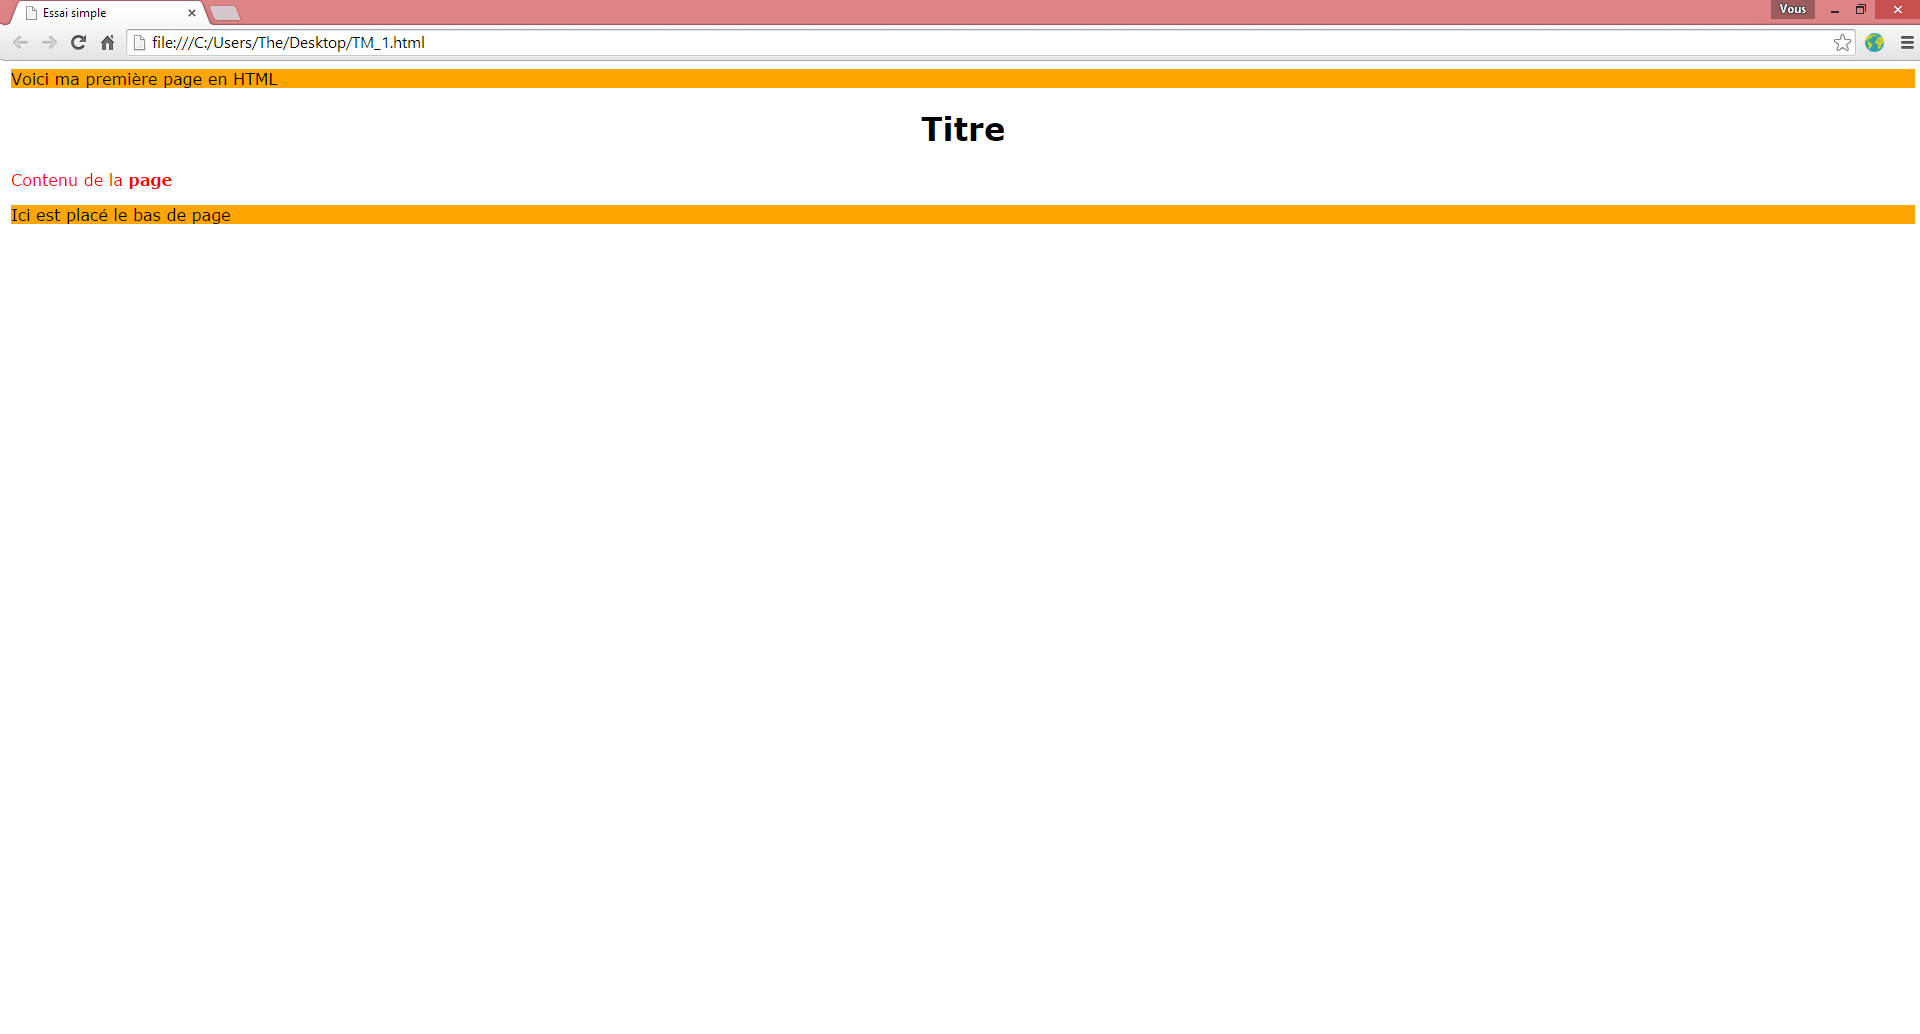
\includegraphics{HTML_presentation_2.png}


\section{Javascript}
\label{technologie:javascript}
Le Javascript est un langage qui lui permet d'ajouter de l'interactivité dans ses
pages internet car comme vous avez pu le remarquer on se retrouve avec des pages
dite `statiques' qui ne font qu'afficher du contenu. Nous allons ici ajouter une
boite de dialogue avec javascript (dans le fichier
javascript.js, chargé dans la page html d'avant):

\begin{Verbatim}[commandchars=\\\{\}]
\PYG{c+cm}{/* la fonction alert permet une boite de dialogue */}
\PYG{n+nx}{alert}\PYG{p}{(}\PYG{l+s+s2}{\PYGZdq{}Ceci est une boite de dialogue à l\PYGZsq{}aide de JS.\PYGZdq{}}\PYG{p}{)}
\end{Verbatim}


\includegraphics{HTML_presentation_3.png}


\section{jQuery}
\label{technologie:jquery}
JQuery est une bibliothèque javascript ce qui veut dire qu'elle est basée sur du
code javascript avec des fonctions déjà préparée et pour pouvoir les utiliser,
nous devons charger un script supplémentaire comme l'on a fait avec le CSS et le
JS:

\begin{Verbatim}[commandchars=\\\{\}]
\PYG{n+nt}{\PYGZlt{}script }\PYG{n+na}{src=}\PYG{l+s}{\PYGZdq{}http://code.jquery.com/jquery\PYGZhy{}1.11.1.min.js\PYGZdq{}}\PYG{n+nt}{\PYGZgt{}}\PYG{n+nt}{\PYGZlt{}/script\PYGZgt{}}
\end{Verbatim}

En plus de cela jQuery utilise également des évènements qui, par exemple, lance
des fonctions lorsqu'on clique sur une bouton. Sur notre page vous avez pu
remarquer que la boite de dialogue s'ouvre avant le chargement de la page. Nous
allons donc remplacer le code javascript d'avant par un autre qui
affichera cette boite de dialogue seulement après le chargement:

\begin{Verbatim}[commandchars=\\\{\}]
\PYG{c+cm}{/* on se réfère au document ouvert, donc la page qui quand elle est prête}
\PYG{c+cm}{méthode \PYGZsq{}ready\PYGZsq{} éxécute la fonction alert que l\PYGZsq{}on a vu précédemment*/}
\PYG{n+nx}{\PYGZdl{}}\PYG{p}{(}\PYG{n+nb}{document}\PYG{p}{)}\PYG{p}{.}\PYG{n+nx}{ready}\PYG{p}{(}\PYG{k+kd}{function}\PYG{p}{(}\PYG{p}{)}\PYG{p}{\PYGZob{}}
    \PYG{n+nx}{alert}\PYG{p}{(}\PYG{l+s+s2}{\PYGZdq{}Voici la nouvelle boite de dialogue.\PYGZdq{}}\PYG{p}{)}\PYG{p}{;}
\PYG{p}{\PYGZcb{}}\PYG{p}{)}\PYG{p}{;}
\end{Verbatim}

Et nous devrions obtenir un résultat de ceci:


\includegraphics{HTML_presentation_4.png}


\section{Django}
\label{technologie:django}
Django est également une bibliothèque mais basée sur le langage python cette fois.
C'est une bibliothèque web qui permet de créer des sites internet de façon plutôt
intuitive une fois que l'on a appréhendé le fonctionnement de celle-ci. Tout
comme python, le langage django est relativement facile à comprendre et permet
de proposer un site web efficace avec un effort qui est moindre.


\section{python}
\label{technologie:python}
Python est donc ce langage qui alimente django et qui lui permet la plupart des
actions. Celui-ci est plutôt de haut niveau ce qui signifie qu'il se rapproche
plutôt de la façon de penser de l'homme plutôt que de la machine. Un petit
exemple qui illustre la syntaxe et l'allure du langage:

\begin{Verbatim}[commandchars=\\\{\}]
\PYG{k}{def} \PYG{n+nf}{somme}\PYG{p}{(}\PYG{n}{nbrUn}\PYG{p}{,} \PYG{n}{nbrDeux}\PYG{p}{)}\PYG{p}{:}
    \PYG{l+s+sd}{\PYGZdq{}\PYGZdq{}\PYGZdq{}somme(float nbrUn, float nbrDeux) \PYGZhy{}\PYGZhy{}\PYGZhy{}\PYGZgt{} float fonction qui retourne}
\PYG{l+s+sd}{    la somme de nbrUn et nbrDeux\PYGZdq{}\PYGZdq{}\PYGZdq{}}
    \PYG{n}{somme} \PYG{o}{=} \PYG{n}{nbrUn} \PYG{o}{+} \PYG{n}{nbrDeux}
    \PYG{k}{return} \PYG{n}{somme}
\end{Verbatim}


\section{jQuery Mobile}
\label{technologie:jquery-mobile}
jquery mobile est cette fameuse bibliothèque que j'aurai l'occasion de présenter
d'une façon plus approfondie dans ce travail. Tout d'abord, il faut la charger
tous les scripts de la même façon que jQuery:

\begin{Verbatim}[commandchars=\\\{\}]
\PYG{c}{\PYGZlt{}!\PYGZhy{}\PYGZhy{}}\PYG{c}{ le script CSS qui va charger les éléments de style jQuery Mobile}\PYG{c}{\PYGZhy{}\PYGZhy{}\PYGZgt{}}

\PYG{n+nt}{\PYGZlt{}link} \PYG{n+na}{rel=}\PYG{l+s}{\PYGZdq{}stylesheet\PYGZdq{}} \PYG{n+na}{href=}\PYG{l+s}{\PYGZdq{}http://code.jquery.com/mobile/1.4.5/jquery.}
\PYG{l+s}{mobile\PYGZhy{}1.4.5.min.css\PYGZdq{}} \PYG{n+nt}{/\PYGZgt{}}

\PYG{c}{\PYGZlt{}!\PYGZhy{}\PYGZhy{}}\PYG{c}{ le script de jQuery qui est aussi nécessaire }\PYG{c}{\PYGZhy{}\PYGZhy{}\PYGZgt{}}
\PYG{n+nt}{\PYGZlt{}script }\PYG{n+na}{src=}\PYG{l+s}{\PYGZdq{}http://code.jquery.com/jquery\PYGZhy{}1.11.1.min.js\PYGZdq{}}\PYG{n+nt}{\PYGZgt{}}\PYG{n+nt}{\PYGZlt{}/script\PYGZgt{}}

\PYG{c}{\PYGZlt{}!\PYGZhy{}\PYGZhy{}}\PYG{c}{ et enfin celui de jQuery Mobile }\PYG{c}{\PYGZhy{}\PYGZhy{}\PYGZgt{}}
\PYG{n+nt}{\PYGZlt{}script }\PYG{n+na}{src=}\PYG{l+s}{\PYGZdq{}http://code.jquery.com/mobile/1.4.5/jquery.mobile\PYGZhy{}1.4.5}
\PYG{l+s}{.min.js\PYGZdq{}}\PYG{n+nt}{\PYGZgt{}}\PYG{n+nt}{\PYGZlt{}/script\PYGZgt{}}
\end{Verbatim}

A partir de là, il ne nous reste plus qu'à retravailler le code html pour
l'adapter au balisage jQuery Mobile. Aussi bien au niveau du nom de la balise,
attribuer un id spécifique ou le plus souvent une classe. Voici une page
jQuery Mobile de base avec un rendu type `écran mobile':

\begin{Verbatim}[commandchars=\\\{\}]
\PYG{c+cp}{\PYGZlt{}!DOCTYPE html\PYGZgt{}}
    \PYG{n+nt}{\PYGZlt{}html}\PYG{n+nt}{\PYGZgt{}}
        \PYG{n+nt}{\PYGZlt{}head}\PYG{n+nt}{\PYGZgt{}}
            \PYG{n+nt}{\PYGZlt{}meta} \PYG{n+na}{charset=}\PYG{l+s}{\PYGZdq{}utf\PYGZhy{}8\PYGZdq{}} \PYG{n+nt}{/\PYGZgt{}}
            \PYG{n+nt}{\PYGZlt{}link} \PYG{n+na}{rel=}\PYG{l+s}{\PYGZdq{}stylesheet\PYGZdq{}} \PYG{n+na}{href=}\PYG{l+s}{\PYGZdq{}http://code.jquery.com/mobile/}
\PYG{l+s}{            1.4.5/jquery.mobile\PYGZhy{}1.4.5.min.css\PYGZdq{}} \PYG{n+nt}{/\PYGZgt{}}
            \PYG{n+nt}{\PYGZlt{}script }\PYG{n+na}{src=}\PYG{l+s}{\PYGZdq{}http://code.jquery.com/jquery\PYGZhy{}1.11.1.min.js\PYGZdq{}}\PYG{n+nt}{\PYGZgt{}}
            \PYG{n+nt}{\PYGZlt{}/script\PYGZgt{}}
            \PYG{n+nt}{\PYGZlt{}script }\PYG{n+na}{src=}\PYG{l+s}{\PYGZdq{}http://code.jquery.com/mobile/1.4.5/jquery.}
\PYG{l+s}{            mobile\PYGZhy{}1.4.5.min.js\PYGZdq{}}\PYG{n+nt}{\PYGZgt{}}\PYG{n+nt}{\PYGZlt{}/script\PYGZgt{}}
                    \PYG{n+nt}{\PYGZlt{}title}\PYG{n+nt}{\PYGZgt{}}Essai simple\PYG{n+nt}{\PYGZlt{}/title\PYGZgt{}}
            \PYG{n+nt}{\PYGZlt{}/head\PYGZgt{}}

            \PYG{n+nt}{\PYGZlt{}body}\PYG{n+nt}{\PYGZgt{}}
                \PYG{c}{\PYGZlt{}!\PYGZhy{}\PYGZhy{}}\PYG{c}{ début de page }\PYG{c}{\PYGZhy{}\PYGZhy{}\PYGZgt{}}
            \PYG{n+nt}{\PYGZlt{}div} \PYG{n+na}{data\PYGZhy{}role=}\PYG{l+s}{\PYGZdq{}page\PYGZdq{}} \PYG{n+na}{id=}\PYG{l+s}{\PYGZdq{}page\PYGZdq{}} \PYG{n+nt}{\PYGZgt{}}

            \PYG{c}{\PYGZlt{}!\PYGZhy{}\PYGZhy{}}\PYG{c}{ début entête }\PYG{c}{\PYGZhy{}\PYGZhy{}\PYGZgt{}}
            \PYG{n+nt}{\PYGZlt{}div} \PYG{n+na}{data\PYGZhy{}role=}\PYG{l+s}{\PYGZdq{}header\PYGZdq{}}\PYG{n+nt}{\PYGZgt{}}
                \PYG{n+nt}{\PYGZlt{}h1}\PYG{n+nt}{\PYGZgt{}}Voici ma première page en HTML\PYG{n+nt}{\PYGZlt{}/h1\PYGZgt{}}
            \PYG{n+nt}{\PYGZlt{}/div\PYGZgt{}}
            \PYG{c}{\PYGZlt{}!\PYGZhy{}\PYGZhy{}}\PYG{c}{ fin entête }\PYG{c}{\PYGZhy{}\PYGZhy{}\PYGZgt{}}

            \PYG{c}{\PYGZlt{}!\PYGZhy{}\PYGZhy{}}\PYG{c}{ début contenu }\PYG{c}{\PYGZhy{}\PYGZhy{}\PYGZgt{}}
            \PYG{n+nt}{\PYGZlt{}div} \PYG{n+na}{role=}\PYG{l+s}{\PYGZdq{}main\PYGZdq{}} \PYG{n+na}{class=}\PYG{l+s}{\PYGZdq{}ui\PYGZhy{}content\PYGZdq{}}\PYG{n+nt}{\PYGZgt{}}
                \PYG{n+nt}{\PYGZlt{}h1}\PYG{n+nt}{\PYGZgt{}}Titre\PYG{n+nt}{\PYGZlt{}/h1\PYGZgt{}}
                    \PYG{n+nt}{\PYGZlt{}p}\PYG{n+nt}{\PYGZgt{}}Contenu de la \PYG{n+nt}{\PYGZlt{}strong}\PYG{n+nt}{\PYGZgt{}}page\PYG{n+nt}{\PYGZlt{}/strong\PYGZgt{}}\PYG{n+nt}{\PYGZlt{}/p\PYGZgt{}}
            \PYG{n+nt}{\PYGZlt{}/div\PYGZgt{}}
            \PYG{c}{\PYGZlt{}!\PYGZhy{}\PYGZhy{}}\PYG{c}{ fin contenu }\PYG{c}{\PYGZhy{}\PYGZhy{}\PYGZgt{}}

            \PYG{c}{\PYGZlt{}!\PYGZhy{}\PYGZhy{}}\PYG{c}{ début bas de page }\PYG{c}{\PYGZhy{}\PYGZhy{}\PYGZgt{}}
            \PYG{n+nt}{\PYGZlt{}div} \PYG{n+na}{data\PYGZhy{}role=}\PYG{l+s}{\PYGZdq{}footer\PYGZdq{}} \PYG{n+na}{data\PYGZhy{}position=}\PYG{l+s}{\PYGZdq{}fixed\PYGZdq{}}\PYG{n+nt}{\PYGZgt{}}
                \PYG{n+nt}{\PYGZlt{}h4}\PYG{n+nt}{\PYGZgt{}}Ici est placé le bas de page\PYG{n+nt}{\PYGZlt{}/h4\PYGZgt{}}
            \PYG{n+nt}{\PYGZlt{}/div\PYGZgt{}}
            \PYG{c}{\PYGZlt{}!\PYGZhy{}\PYGZhy{}}\PYG{c}{ fin bas de page }\PYG{c}{\PYGZhy{}\PYGZhy{}\PYGZgt{}}

            \PYG{n+nt}{\PYGZlt{}/div\PYGZgt{}}
            \PYG{c}{\PYGZlt{}!\PYGZhy{}\PYGZhy{}}\PYG{c}{ fin de page }\PYG{c}{\PYGZhy{}\PYGZhy{}\PYGZgt{}}
            \PYG{n+nt}{\PYGZlt{}/body\PYGZgt{}}
    \PYG{n+nt}{\PYGZlt{}/html\PYGZgt{}}
\end{Verbatim}

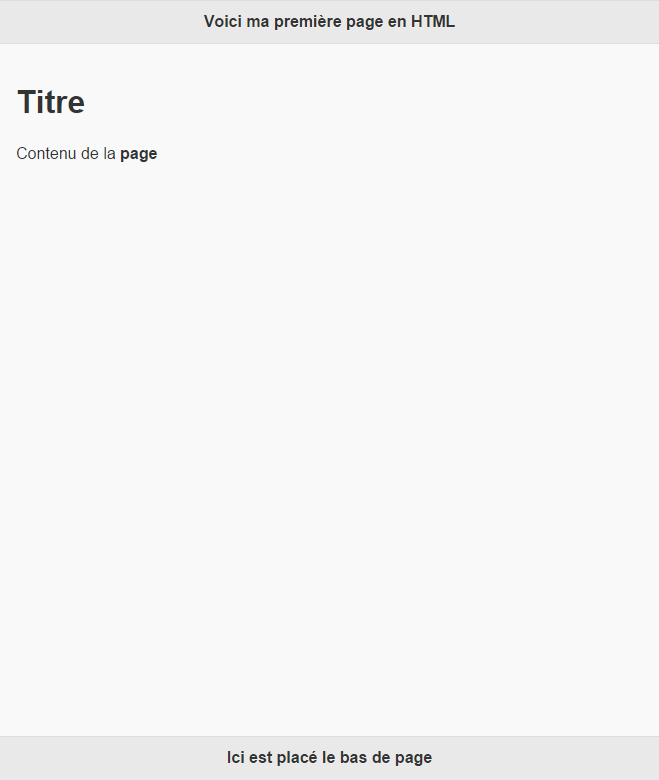
\includegraphics{HTML_presentation_5.png}

On voit déjà ici la puissance de jQuery Mobile pour la mise en page qui malgré
son thème de base reste très agréable et s'adapte bien au petits écrans.


\chapter{Guide du programmeur}
\label{guide::doc}\label{guide:guide-du-programmeur}

\section{Introduction}
\label{guide:introduction}
Dans ce guide du programmeur, je vais vous montrer comment coder une application
web qui permet de charger des images sur un serveur. Ce tutoriel prend en compte
que vous connaissez un minimum django, le HTML et le CSS.


\section{Les modèles}
\label{guide:les-modeles}
Après avoir créé l'application django et réglé le nécessaire dans django, nous
allons commencer par les modèles dans le fichier `models.py':

\begin{Verbatim}[commandchars=\\\{\}]
\PYG{k+kn}{from} \PYG{n+nn}{django.db} \PYG{k+kn}{import} \PYG{n}{models}

\PYG{k}{class} \PYG{n+nc}{Picture}\PYG{p}{(}\PYG{n}{models}\PYG{o}{.}\PYG{n}{Model}\PYG{p}{)}\PYG{p}{:}
    \PYG{c}{\PYGZsh{}ImageField pour que l\PYGZsq{}image soit enregistrée comme une image}
    \PYG{n}{image} \PYG{o}{=} \PYG{n}{models}\PYG{o}{.}\PYG{n}{ImageField}\PYG{p}{(}\PYG{n}{upload\PYGZus{}to}\PYG{o}{=}\PYG{l+s}{\PYGZdq{}}\PYG{l+s}{uploadedImages}\PYG{l+s}{\PYGZdq{}}\PYG{p}{)}

    \PYG{c}{\PYGZsh{}tag: court énoncé sur l\PYGZsq{}image}
    \PYG{n}{tag} \PYG{o}{=} \PYG{n}{models}\PYG{o}{.}\PYG{n}{CharField}\PYG{p}{(}\PYG{n}{max\PYGZus{}length}\PYG{o}{=}\PYG{l+m+mi}{20}\PYG{p}{)}

    \PYG{c}{\PYGZsh{}description: texte pour décrire l\PYGZsq{}image}
    \PYG{n}{description} \PYG{o}{=} \PYG{n}{models}\PYG{o}{.}\PYG{n}{CharField}\PYG{p}{(}\PYG{n}{max\PYGZus{}length}\PYG{o}{=}\PYG{l+m+mi}{500}\PYG{p}{)}

    \PYG{c}{\PYGZsh{}date de l\PYGZsq{}upload}
    \PYG{n}{date} \PYG{o}{=} \PYG{n}{models}\PYG{o}{.}\PYG{n}{DateField}\PYG{p}{(}\PYG{n}{auto\PYGZus{}now\PYGZus{}add}\PYG{o}{=}\PYG{n+nb+bp}{True}\PYG{p}{)}
\end{Verbatim}

Ensuite, on procède au fameux ` makemigrations \textless{}nomApp\textgreater{} ` et ` migrate `


\section{Les formulaires}
\label{guide:les-formulaires}
Les formulaires sont indispensables lorsque l'on veut charger une image ou du
texte sur un serveur et que l'on désire contrôler si ce que l'utilisateur a
saisi est bien le type de données qui est attendu nous créons alors ces
formulaires dans le fichier `forms.py':

\begin{Verbatim}[commandchars=\\\{\}]
\PYG{k+kn}{from} \PYG{n+nn}{django} \PYG{k+kn}{import} \PYG{n}{forms}

\PYG{c}{\PYGZsh{}classe pour le téléversement d\PYGZsq{}images}
\PYG{k}{class} \PYG{n+nc}{ChargementForm}\PYG{p}{(}\PYG{n}{forms}\PYG{o}{.}\PYG{n}{Form}\PYG{p}{)}\PYG{p}{:}
    \PYG{n}{image} \PYG{o}{=} \PYG{n}{forms}\PYG{o}{.}\PYG{n}{ImageField}\PYG{p}{(}\PYG{p}{)}
    \PYG{n}{tag} \PYG{o}{=} \PYG{n}{forms}\PYG{o}{.}\PYG{n}{CharField}\PYG{p}{(}\PYG{n}{max\PYGZus{}length}\PYG{o}{=}\PYG{l+m+mi}{20}\PYG{p}{)}
    \PYG{n}{description} \PYG{o}{=} \PYG{n}{forms}\PYG{o}{.}\PYG{n}{CharField}\PYG{p}{(}\PYG{n}{max\PYGZus{}length}\PYG{o}{=}\PYG{l+m+mi}{500}\PYG{p}{)}

\PYG{c}{\PYGZsh{}classe pour le formulaire de modifications}
\PYG{k}{class} \PYG{n+nc}{ModificationForm}\PYG{p}{(}\PYG{n}{forms}\PYG{o}{.}\PYG{n}{Form}\PYG{p}{)}\PYG{p}{:}
    \PYG{n}{tag} \PYG{o}{=} \PYG{n}{forms}\PYG{o}{.}\PYG{n}{CharField}\PYG{p}{(}\PYG{n}{max\PYGZus{}length}\PYG{o}{=}\PYG{l+m+mi}{20}\PYG{p}{)}
    \PYG{n}{description} \PYG{o}{=} \PYG{n}{forms}\PYG{o}{.}\PYG{n}{CharField}\PYG{p}{(}\PYG{n}{max\PYGZus{}length}\PYG{o}{=}\PYG{l+m+mi}{500}\PYG{p}{)}
\end{Verbatim}

On observe une forte similairité avec les classes de modèles. Ceci est dû au
fait que les formulaire sont créés pour instancier des objets des classes des
modèles.


\section{Les vues}
\label{guide:les-vues}
Ici nous allons créer quelques vues qui serviront à charger l'image sur le
serveur, supprimer l'image, afficher toutes les images ou encore modifier
les détails d'une image.

\begin{Verbatim}[commandchars=\\\{\}]
\PYG{k+kn}{from} \PYG{n+nn}{django.shortcuts} \PYG{k+kn}{import} \PYG{n}{render}\PYG{p}{,} \PYG{n}{redirect}
\PYG{k+kn}{from} \PYG{o}{\PYGZlt{}}\PYG{n}{nomApp}\PYG{o}{\PYGZgt{}}\PYG{o}{.}\PYG{n}{forms} \PYG{k+kn}{import} \PYG{n+nn}{ChargementForm}\PYG{o}{,} \PYG{n+nn}{ModificationForm}
\PYG{k+kn}{from} \PYG{o}{\PYGZlt{}}\PYG{n}{nomApp}\PYG{o}{\PYGZgt{}}\PYG{o}{.}\PYG{n}{models} \PYG{k+kn}{import} \PYG{n+nn}{Picture}

\PYG{c}{\PYGZsh{}vue pour charger une image sur le serveur, si la requête post a lieu et que}
\PYG{c}{\PYGZsh{}tous les champs du formulaire sont correctement remplis, on sauvegarde cette}
\PYG{c}{\PYGZsh{}instance. Le boléen sauvegarde sera utile pour affiche un message lorsque}
\PYG{c}{\PYGZsh{}l\PYGZsq{}image aura été chargée.}
\PYG{k}{def} \PYG{n+nf}{chargement}\PYG{p}{(}\PYG{n}{request}\PYG{p}{)}\PYG{p}{:}
    \PYG{n}{sauvegarde} \PYG{o}{=} \PYG{n+nb+bp}{False}

    \PYG{k}{if} \PYG{n}{request}\PYG{o}{.}\PYG{n}{method} \PYG{o}{==} \PYG{l+s}{\PYGZdq{}}\PYG{l+s}{POST}\PYG{l+s}{\PYGZdq{}}\PYG{p}{:}
        \PYG{n}{form} \PYG{o}{=} \PYG{n}{ChargementForm}\PYG{p}{(}\PYG{n}{request}\PYG{o}{.}\PYG{n}{POST}\PYG{p}{,} \PYG{n}{request}\PYG{o}{.}\PYG{n}{FILES}\PYG{p}{)}
        \PYG{k}{if} \PYG{n}{form}\PYG{o}{.}\PYG{n}{is\PYGZus{}valid}\PYG{p}{(}\PYG{p}{)}\PYG{p}{:}
            \PYG{n}{image} \PYG{o}{=} \PYG{n}{Picture}\PYG{p}{(}\PYG{p}{)}
            \PYG{n}{image}\PYG{o}{.}\PYG{n}{image} \PYG{o}{=} \PYG{n}{form}\PYG{o}{.}\PYG{n}{cleaned\PYGZus{}data}\PYG{p}{[}\PYG{l+s}{\PYGZdq{}}\PYG{l+s}{image}\PYG{l+s}{\PYGZdq{}}\PYG{p}{]}
            \PYG{n}{image}\PYG{o}{.}\PYG{n}{tag} \PYG{o}{=} \PYG{n}{form}\PYG{o}{.}\PYG{n}{cleaned\PYGZus{}data}\PYG{p}{[}\PYG{l+s}{\PYGZdq{}}\PYG{l+s}{tag}\PYG{l+s}{\PYGZdq{}}\PYG{p}{]}
            \PYG{n}{image}\PYG{o}{.}\PYG{n}{description} \PYG{o}{=} \PYG{n}{form}\PYG{o}{.}\PYG{n}{cleaned\PYGZus{}data}\PYG{p}{[}\PYG{l+s}{\PYGZdq{}}\PYG{l+s}{description}\PYG{l+s}{\PYGZdq{}}\PYG{p}{]}
            \PYG{n}{image}\PYG{o}{.}\PYG{n}{save}\PYG{p}{(}\PYG{p}{)}
            \PYG{n}{sauvegarde} \PYG{o}{=} \PYG{n+nb+bp}{True}
    \PYG{k}{else}\PYG{p}{:}
        \PYG{n}{form} \PYG{o}{=} \PYG{n}{ChargementForm}\PYG{p}{(}\PYG{p}{)}

    \PYG{k}{return} \PYG{n}{render}\PYG{p}{(}\PYG{n}{request}\PYG{p}{,} \PYG{l+s}{\PYGZsq{}}\PYG{l+s}{chargement.html}\PYG{l+s}{\PYGZsq{}}\PYG{p}{,} \PYG{n+nb}{locals}\PYG{p}{(}\PYG{p}{)}\PYG{p}{)}

\PYG{c}{\PYGZsh{}vue pour afficher toutes les images. On instancie tous les objets de la}
\PYG{c}{\PYGZsh{}classe Picture et on retourne le template et les images}
\PYG{k}{def} \PYG{n+nf}{index}\PYG{p}{(}\PYG{n}{request}\PYG{p}{)}\PYG{p}{:}
    \PYG{n}{images} \PYG{o}{=} \PYG{n}{Picture}\PYG{o}{.}\PYG{n}{objects}\PYG{o}{.}\PYG{n}{all}\PYG{p}{(}\PYG{p}{)}
    \PYG{k}{return} \PYG{n}{render}\PYG{p}{(}\PYG{n}{request}\PYG{p}{,} \PYG{l+s}{\PYGZsq{}}\PYG{l+s}{index\PYGZus{}images.html}\PYG{l+s}{\PYGZsq{}}\PYG{p}{,} \PYG{p}{\PYGZob{}}\PYG{l+s}{\PYGZsq{}}\PYG{l+s}{images}\PYG{l+s}{\PYGZsq{}}\PYG{p}{:} \PYG{n}{images}\PYG{p}{\PYGZcb{}}\PYG{p}{)}

\PYG{c}{\PYGZsh{}vue pour afficher le détail d\PYGZsq{}une image. On instancie l\PYGZsq{}objet de la classe}
\PYG{c}{\PYGZsh{}picture qui correspond a l\PYGZsq{}id désiré (récupéré dans l\PYGZsq{}url) et l\PYGZsq{}on retourne}
\PYG{c}{\PYGZsh{}le template, l\PYGZsq{}instanciation d\PYGZsq{}image et de formulaire grâce à \PYGZsq{}locals()\PYGZsq{}}
\PYG{k}{def} \PYG{n+nf}{detail\PYGZus{}image}\PYG{p}{(}\PYG{n}{request}\PYG{p}{,} \PYG{n}{imageId}\PYG{p}{)}\PYG{p}{:}
    \PYG{n}{image} \PYG{o}{=} \PYG{n}{Picture}\PYG{o}{.}\PYG{n}{objects}\PYG{o}{.}\PYG{n}{get}\PYG{p}{(}\PYG{n+nb}{id}\PYG{o}{=}\PYG{n}{imageId}\PYG{p}{)}
    \PYG{n}{form} \PYG{o}{=} \PYG{n}{ModificationForm}\PYG{p}{(}\PYG{p}{)}
    \PYG{k}{return} \PYG{n}{render}\PYG{p}{(}\PYG{n}{request}\PYG{p}{,} \PYG{l+s}{\PYGZsq{}}\PYG{l+s}{image\PYGZus{}detail.html}\PYG{l+s}{\PYGZsq{}}\PYG{p}{,} \PYG{n+nb}{locals}\PYG{p}{(}\PYG{p}{)}\PYG{p}{)}

\PYG{c}{\PYGZsh{}vue pour supprimer une image, active lors d\PYGZsq{}une requête post et qui supprime}
\PYG{c}{\PYGZsh{}l\PYGZsq{}image elle\PYGZhy{}même ainsi que l\PYGZsq{}instance de la classe Picture avant de nous}
\PYG{c}{\PYGZsh{}rediriger vers l\PYGZsq{}index}
\PYG{k}{def} \PYG{n+nf}{supprimer\PYGZus{}image}\PYG{p}{(}\PYG{n}{request}\PYG{p}{,} \PYG{n}{imageId}\PYG{p}{)}\PYG{p}{:}
    \PYG{k}{if} \PYG{n}{request}\PYG{o}{.}\PYG{n}{method} \PYG{o}{==} \PYG{l+s}{\PYGZdq{}}\PYG{l+s}{POST}\PYG{l+s}{\PYGZdq{}}\PYG{p}{:}
        \PYG{n}{image} \PYG{o}{=} \PYG{n}{Picture}\PYG{o}{.}\PYG{n}{objects}\PYG{o}{.}\PYG{n}{get}\PYG{p}{(}\PYG{n+nb}{id}\PYG{o}{=}\PYG{n}{imageId}\PYG{p}{)}
        \PYG{n}{image}\PYG{o}{.}\PYG{n}{image}\PYG{o}{.}\PYG{n}{delete}\PYG{p}{(}\PYG{p}{)}
        \PYG{n}{image}\PYG{o}{.}\PYG{n}{delete}\PYG{p}{(}\PYG{p}{)}
        \PYG{k}{return} \PYG{n}{redirect}\PYG{p}{(}\PYG{l+s}{\PYGZsq{}}\PYG{l+s}{\PYGZlt{}nomApp\PYGZgt{}:index}\PYG{l+s}{\PYGZsq{}}\PYG{p}{)}

\PYG{c}{\PYGZsh{}vue pour modifier le tag ou la description d\PYGZsq{}une image, il s\PYGZsq{}agit du même}
\PYG{c}{\PYGZsh{}principe que les vues d\PYGZsq{}avant.}
\PYG{k}{def} \PYG{n+nf}{modifier\PYGZus{}image}\PYG{p}{(}\PYG{n}{request}\PYG{p}{,} \PYG{n}{imageId}\PYG{p}{)}\PYG{p}{:}
    \PYG{n}{image} \PYG{o}{=} \PYG{n}{Picture}\PYG{o}{.}\PYG{n}{objects}\PYG{o}{.}\PYG{n}{get}\PYG{p}{(}\PYG{n+nb}{id}\PYG{o}{=}\PYG{n}{imageId}\PYG{p}{)}
    \PYG{k}{if} \PYG{n}{request}\PYG{o}{.}\PYG{n}{method} \PYG{o}{==} \PYG{l+s}{\PYGZdq{}}\PYG{l+s}{POST}\PYG{l+s}{\PYGZdq{}}\PYG{p}{:}
        \PYG{n}{form} \PYG{o}{=} \PYG{n}{ModificationForm}\PYG{p}{(}\PYG{n}{request}\PYG{o}{.}\PYG{n}{POST}\PYG{p}{,} \PYG{n}{request}\PYG{o}{.}\PYG{n}{FILES}\PYG{p}{)}
        \PYG{k}{if} \PYG{n}{form}\PYG{o}{.}\PYG{n}{is\PYGZus{}valid}\PYG{p}{(}\PYG{p}{)}\PYG{p}{:}
            \PYG{n}{image}\PYG{o}{.}\PYG{n}{tag} \PYG{o}{=} \PYG{n}{form}\PYG{o}{.}\PYG{n}{cleaned\PYGZus{}data}\PYG{p}{[}\PYG{l+s}{\PYGZdq{}}\PYG{l+s}{tag}\PYG{l+s}{\PYGZdq{}}\PYG{p}{]}
            \PYG{n}{image}\PYG{o}{.}\PYG{n}{description} \PYG{o}{=} \PYG{n}{form}\PYG{o}{.}\PYG{n}{cleaned\PYGZus{}data}\PYG{p}{[}\PYG{l+s}{\PYGZdq{}}\PYG{l+s}{description}\PYG{l+s}{\PYGZdq{}}\PYG{p}{]}
            \PYG{n}{image}\PYG{o}{.}\PYG{n}{save}\PYG{p}{(}\PYG{p}{)}
            \PYG{k}{return} \PYG{n}{redirect}\PYG{p}{(}\PYG{l+s}{\PYGZsq{}}\PYG{l+s}{\PYGZlt{}nomApp\PYGZgt{}:index}\PYG{l+s}{\PYGZsq{}}\PYG{p}{)}
        \PYG{k}{else}\PYG{p}{:}
            \PYG{k}{return} \PYG{n}{redirect}\PYG{p}{(}\PYG{l+s}{\PYGZsq{}}\PYG{l+s}{\PYGZlt{}nomApp\PYGZgt{}:index}\PYG{l+s}{\PYGZsq{}}\PYG{p}{)}
\end{Verbatim}


\section{Fichier settings.py}
\label{guide:fichier-settings-py}
Pour que les images soit enregistrées correctement il est nécessaire de définir
ces variables là:

\begin{Verbatim}[commandchars=\\\{\}]
\PYG{n}{MEDIA\PYGZus{}ROOT} \PYG{o}{=} \PYG{n}{os}\PYG{o}{.}\PYG{n}{path}\PYG{o}{.}\PYG{n}{join}\PYG{p}{(}\PYG{n}{BASE\PYGZus{}DIR}\PYG{p}{,} \PYG{l+s}{\PYGZsq{}}\PYG{l+s}{media/}\PYG{l+s}{\PYGZsq{}}\PYG{p}{)}
\PYG{n}{MEDIA\PYGZus{}URL} \PYG{o}{=} \PYG{n}{os}\PYG{o}{.}\PYG{n}{path}\PYG{o}{.}\PYG{n}{join}\PYG{p}{(}\PYG{n}{BASE\PYGZus{}DIR}\PYG{p}{,} \PYG{l+s}{\PYGZsq{}}\PYG{l+s}{media/}\PYG{l+s}{\PYGZsq{}}\PYG{p}{)}
\end{Verbatim}


\section{Fichier urls.py}
\label{guide:fichier-urls-py}
Nous devons d'abord ajouter le chemin vers les urls de l'application que nous
avons créée. Ceci doit dans le fichier urls.py dans les fichiers de
l'environnement de travail, ce ne sont pas les urls.py spécifique à
l'application que nous sommes en train de créer):

\begin{Verbatim}[commandchars=\\\{\}]
\PYG{k+kn}{from} \PYG{n+nn}{django.conf.urls} \PYG{k+kn}{import} \PYG{n}{patterns}\PYG{p}{,} \PYG{n}{include}\PYG{p}{,} \PYG{n}{url}
\PYG{k+kn}{from} \PYG{n+nn}{django.contrib} \PYG{k+kn}{import} \PYG{n}{admin}
\PYG{k+kn}{from} \PYG{n+nn}{django.conf.urls.static} \PYG{k+kn}{import} \PYG{n}{static}
\PYG{k+kn}{from} \PYG{n+nn}{django.conf} \PYG{k+kn}{import} \PYG{n}{settings}

\PYG{n}{urlpatterns} \PYG{o}{=} \PYG{n}{patterns}\PYG{p}{(}\PYG{l+s}{\PYGZsq{}}\PYG{l+s}{\PYGZsq{}}\PYG{p}{,}
    \PYG{n}{url}\PYG{p}{(}\PYG{l+s}{r\PYGZsq{}}\PYG{l+s}{\PYGZca{}admin/}\PYG{l+s}{\PYGZsq{}}\PYG{p}{,} \PYG{n}{include}\PYG{p}{(}\PYG{n}{admin}\PYG{o}{.}\PYG{n}{site}\PYG{o}{.}\PYG{n}{urls}\PYG{p}{)}\PYG{p}{)}\PYG{p}{,}
    \PYG{c}{\PYGZsh{}cette ligne\PYGZhy{}ci}
    \PYG{n}{url}\PYG{p}{(}\PYG{l+s}{r\PYGZsq{}}\PYG{l+s}{\PYGZca{}\PYGZlt{}nomApp\PYGZgt{}/}\PYG{l+s}{\PYGZsq{}}\PYG{p}{,} \PYG{n}{include}\PYG{p}{(}\PYG{l+s}{\PYGZsq{}}\PYG{l+s}{\PYGZlt{}nomApp\PYGZgt{}.urls}\PYG{l+s}{\PYGZsq{}}\PYG{p}{,} \PYG{n}{namespace}\PYG{o}{=}\PYG{l+s}{\PYGZdq{}}\PYG{l+s}{\PYGZlt{}nomApp\PYGZgt{}}\PYG{l+s}{\PYGZdq{}}\PYG{p}{)}\PYG{p}{)}\PYG{p}{,}
\PYG{p}{)}

\PYG{c}{\PYGZsh{}Et l\PYGZsq{}ajout de cette ligne également pour l\PYGZsq{}accès aux images chargées}
\PYG{n}{urlpatterns} \PYG{o}{+}\PYG{o}{=} \PYG{n}{static}\PYG{p}{(}\PYG{n}{settings}\PYG{o}{.}\PYG{n}{MEDIA\PYGZus{}URL}\PYG{p}{,} \PYG{n}{document\PYGZus{}root}\PYG{o}{=}\PYG{n}{settings}\PYG{o}{.}\PYG{n}{MEDIA\PYGZus{}ROOT}\PYG{p}{)}
\end{Verbatim}

Nous devons aussi créer nos propres url pour l'application que nous sommes en
train de creer dans le fichiers urls.py de l'application:

\begin{Verbatim}[commandchars=\\\{\}]
\PYG{k+kn}{from} \PYG{n+nn}{django.conf.urls} \PYG{k+kn}{import} \PYG{n}{patterns}\PYG{p}{,} \PYG{n}{url}
\PYG{k+kn}{from} \PYG{n+nn}{django.conf} \PYG{k+kn}{import} \PYG{n}{settings}
\PYG{k+kn}{from} \PYG{n+nn}{django.conf.urls.static} \PYG{k+kn}{import} \PYG{n}{static}

\PYG{k+kn}{from} \PYG{o}{\PYGZlt{}}\PYG{n}{nomApp}\PYG{o}{\PYGZgt{}} \PYG{k+kn}{import} \PYG{n+nn}{views}

\PYG{n}{urlpatterns} \PYG{o}{=} \PYG{n}{patterns}\PYG{p}{(}\PYG{l+s}{\PYGZsq{}}\PYG{l+s}{\PYGZsq{}}\PYG{p}{,}

    \PYG{c}{\PYGZsh{}pour la vue d\PYGZsq{}index}
    \PYG{n}{url}\PYG{p}{(}\PYG{l+s}{r\PYGZsq{}}\PYG{l+s}{\PYGZca{}index/}\PYG{l+s}{\PYGZsq{}}\PYG{p}{,} \PYG{n}{views}\PYG{o}{.}\PYG{n}{index}\PYG{p}{,} \PYG{n}{name}\PYG{o}{=}\PYG{l+s}{\PYGZsq{}}\PYG{l+s}{index}\PYG{l+s}{\PYGZsq{}}\PYG{p}{)}\PYG{p}{,}

    \PYG{c}{\PYGZsh{}pour la vue détaillée}
    \PYG{n}{url}\PYG{p}{(}\PYG{l+s}{r\PYGZsq{}}\PYG{l+s}{detail/(?P\PYGZlt{}imageId\PYGZgt{}}\PYG{l+s}{\PYGZbs{}}\PYG{l+s}{w+)}\PYG{l+s}{\PYGZsq{}}\PYG{p}{,} \PYG{n}{views}\PYG{o}{.}\PYG{n}{detail\PYGZus{}image}\PYG{p}{,} \PYG{n}{name}\PYG{o}{=}\PYG{l+s}{\PYGZsq{}}\PYG{l+s}{detail\PYGZus{}image}\PYG{l+s}{\PYGZsq{}}\PYG{p}{)}\PYG{p}{,}

    \PYG{c}{\PYGZsh{}pour la vue de chargement}
    \PYG{n}{url}\PYG{p}{(}\PYG{l+s}{r\PYGZsq{}}\PYG{l+s}{\PYGZca{}chargement/}\PYG{l+s}{\PYGZsq{}}\PYG{p}{,} \PYG{n}{views}\PYG{o}{.}\PYG{n}{chargement}\PYG{p}{,} \PYG{n}{name}\PYG{o}{=}\PYG{l+s}{\PYGZsq{}}\PYG{l+s}{chargement}\PYG{l+s}{\PYGZsq{}}\PYG{p}{)}\PYG{p}{,}

    \PYG{c}{\PYGZsh{}suppression d\PYGZsq{}image}
    \PYG{n}{url}\PYG{p}{(}\PYG{l+s}{r\PYGZsq{}}\PYG{l+s}{suppression/(?P\PYGZlt{}imageId\PYGZgt{}}\PYG{l+s}{\PYGZbs{}}\PYG{l+s}{w+)}\PYG{l+s}{\PYGZsq{}}\PYG{p}{,} \PYG{n}{views}\PYG{o}{.}\PYG{n}{supprimer\PYGZus{}image}\PYG{p}{,} \PYG{n}{name}\PYG{o}{=}\PYG{l+s}{\PYGZsq{}}\PYG{l+s}{supprimer\PYGZus{}image}\PYG{l+s}{\PYGZsq{}}\PYG{p}{)}\PYG{p}{,}

    \PYG{c}{\PYGZsh{}modification d\PYGZsq{}image}
    \PYG{n}{url}\PYG{p}{(}\PYG{l+s}{r\PYGZsq{}}\PYG{l+s}{modification/(?P\PYGZlt{}imageId\PYGZgt{}}\PYG{l+s}{\PYGZbs{}}\PYG{l+s}{w+)}\PYG{l+s}{\PYGZsq{}}\PYG{p}{,} \PYG{n}{views}\PYG{o}{.}\PYG{n}{modifier\PYGZus{}image}\PYG{p}{,} \PYG{n}{name}\PYG{o}{=}\PYG{l+s}{\PYGZsq{}}\PYG{l+s}{modifier\PYGZus{}image}\PYG{l+s}{\PYGZsq{}}\PYG{p}{)}\PYG{p}{,}
\PYG{p}{)}
\end{Verbatim}


\section{Les templates}
\label{guide:les-templates}
Nous avons déjà préparé toute la partie cachée qui va s'éxécuter lorsque l'on
utilisera notr application mais nous n'avons encore fait aucune page qui nous
permettra d'utiliser toutes ces fonctions, nous allons donc nous attaquer aux
templates. Les templates présentés sont composés d'éléments de jQuery Mobile,
qui seront précisément présentés lors de la démostration des fonctionnalités de
mon application utilisée dans sa version finale.

Nous utiliserons la balise blocks pour notre premier template :base.html':

Ne pas oublier dans un premier temps d'ajouter la directions vers le dossier où
se trouvent les templates:

\begin{Verbatim}[commandchars=\\\{\}]
\PYG{n}{TEMPLATE\PYGZus{}DIRS} \PYG{o}{=} \PYG{p}{[}\PYG{n}{os}\PYG{o}{.}\PYG{n}{path}\PYG{o}{.}\PYG{n}{join}\PYG{p}{(}\PYG{n}{BASE\PYGZus{}DIR}\PYG{p}{,} \PYG{l+s}{\PYGZsq{}}\PYG{l+s}{templates}\PYG{l+s}{\PYGZsq{}}\PYG{p}{)}\PYG{p}{]}
\end{Verbatim}

Ensuite placer le fichier `base.hmtl' dans ce même dossier:

\begin{Verbatim}[commandchars=\\\{\}]
\PYG{c+cp}{\PYGZlt{}!DOCTYPE html\PYGZgt{}}
\PYG{n+nt}{\PYGZlt{}html}\PYG{n+nt}{\PYGZgt{}}
    \PYG{n+nt}{\PYGZlt{}head}\PYG{n+nt}{\PYGZgt{}}
        \PYG{n+nt}{\PYGZlt{}meta} \PYG{n+na}{charset=}\PYG{l+s}{\PYGZdq{}utf\PYGZhy{}8\PYGZdq{}} \PYG{n+nt}{/\PYGZgt{}}
        \PYG{n+nt}{\PYGZlt{}title}\PYG{n+nt}{\PYGZgt{}}Mobile\PYG{n+nt}{\PYGZlt{}/title\PYGZgt{}}
        \PYG{c}{\PYGZlt{}!\PYGZhy{}\PYGZhy{}}\PYG{c}{ ligne pour que le contenu s\PYGZsq{}adapte à l\PYGZsq{}appreil mobile }\PYG{c}{\PYGZhy{}\PYGZhy{}\PYGZgt{}}
        \PYG{n+nt}{\PYGZlt{}meta} \PYG{n+na}{name=}\PYG{l+s}{\PYGZdq{}viewport\PYGZdq{}} \PYG{n+na}{content=}\PYG{l+s}{\PYGZdq{}width=device\PYGZhy{}width, initial\PYGZhy{}scale=1\PYGZdq{}}\PYG{n+nt}{\PYGZgt{}}
        \PYG{c}{\PYGZlt{}!\PYGZhy{}\PYGZhy{}}\PYG{c}{ chargement des script et du css nécessaire }\PYG{c}{\PYGZhy{}\PYGZhy{}\PYGZgt{}}
        \PYGZob{}\PYGZpc{} load staticfiles \PYGZpc{}\PYGZcb{}
        \PYG{c}{\PYGZlt{}!\PYGZhy{}\PYGZhy{}}\PYG{c}{ cdn jqm et jq }\PYG{c}{\PYGZhy{}\PYGZhy{}\PYGZgt{}}
        \PYG{n+nt}{\PYGZlt{}link} \PYG{n+na}{rel=}\PYG{l+s}{\PYGZdq{}stylesheet\PYGZdq{}} \PYG{n+na}{href=}\PYG{l+s}{\PYGZdq{}http://code.jquery.com/mobile/}
\PYG{l+s}{        1.4.5/jquery.mobile\PYGZhy{}1.4.5.min.css\PYGZdq{}} \PYG{n+nt}{/\PYGZgt{}}
        \PYG{n+nt}{\PYGZlt{}script }\PYG{n+na}{src=}\PYG{l+s}{\PYGZdq{}http://code.jquery.com/jquery\PYGZhy{}1.11.1.min.js\PYGZdq{}}\PYG{n+nt}{\PYGZgt{}}\PYG{n+nt}{\PYGZlt{}/script\PYGZgt{}}
        \PYG{n+nt}{\PYGZlt{}script }\PYG{n+na}{src=}\PYG{l+s}{\PYGZdq{}http://code.jquery.com/mobile/}
\PYG{l+s}{        1.4.5/jquery.mobile\PYGZhy{}1.4.5.min.js\PYGZdq{}}\PYG{n+nt}{\PYGZgt{}}\PYG{n+nt}{\PYGZlt{}/script\PYGZgt{}}
    \PYG{n+nt}{\PYGZlt{}/head\PYGZgt{}}
    \PYG{n+nt}{\PYGZlt{}body}\PYG{n+nt}{\PYGZgt{}}
        \PYG{c}{\PYGZlt{}!\PYGZhy{}\PYGZhy{}}\PYG{c}{ début de page }\PYG{c}{\PYGZhy{}\PYGZhy{}\PYGZgt{}}
        \PYG{n+nt}{\PYGZlt{}div} \PYG{n+na}{data\PYGZhy{}role=}\PYG{l+s}{\PYGZdq{}page\PYGZdq{}}\PYG{n+nt}{\PYGZgt{}}
        \PYG{c}{\PYGZlt{}!\PYGZhy{}\PYGZhy{}}\PYG{c}{ début entête }\PYG{c}{\PYGZhy{}\PYGZhy{}\PYGZgt{}}
        \PYG{n+nt}{\PYGZlt{}div} \PYG{n+na}{data\PYGZhy{}role=}\PYG{l+s}{\PYGZdq{}header\PYGZdq{}}\PYG{n+nt}{\PYGZgt{}}
        \PYG{n+nt}{\PYGZlt{}h1}\PYG{n+nt}{\PYGZgt{}}MonApp\PYG{n+nt}{\PYGZlt{}/h1\PYGZgt{}}
        \PYG{n+nt}{\PYGZlt{}/div\PYGZgt{}}
        \PYG{c}{\PYGZlt{}!\PYGZhy{}\PYGZhy{}}\PYG{c}{ fin entête }\PYG{c}{\PYGZhy{}\PYGZhy{}\PYGZgt{}}

        \PYG{c}{\PYGZlt{}!\PYGZhy{}\PYGZhy{}}\PYG{c}{ début contenu }\PYG{c}{\PYGZhy{}\PYGZhy{}\PYGZgt{}}
        \PYG{n+nt}{\PYGZlt{}div} \PYG{n+na}{role=}\PYG{l+s}{\PYGZdq{}main\PYGZdq{}} \PYG{n+na}{class=}\PYG{l+s}{\PYGZdq{}ui\PYGZhy{}content\PYGZdq{}}\PYG{n+nt}{\PYGZgt{}}
        \PYGZob{}\PYGZpc{} block content \PYGZpc{}\PYGZcb{}\PYG{n+nt}{\PYGZlt{}p}\PYG{n+nt}{\PYGZgt{}}Content\PYG{n+nt}{\PYGZlt{}/p\PYGZgt{}}\PYGZob{}\PYGZpc{} endblock \PYGZpc{}\PYGZcb{}
        \PYG{n+nt}{\PYGZlt{}/div\PYGZgt{}}
        \PYG{c}{\PYGZlt{}!\PYGZhy{}\PYGZhy{}}\PYG{c}{ fin contenu }\PYG{c}{\PYGZhy{}\PYGZhy{}\PYGZgt{}}

        \PYG{c}{\PYGZlt{}!\PYGZhy{}\PYGZhy{}}\PYG{c}{ début bas de page }\PYG{c}{\PYGZhy{}\PYGZhy{}\PYGZgt{}}
        \PYG{n+nt}{\PYGZlt{}div} \PYG{n+na}{data\PYGZhy{}role=}\PYG{l+s}{\PYGZdq{}footer\PYGZdq{}}\PYG{n+nt}{\PYGZgt{}}
        \PYG{n+nt}{\PYGZlt{}h4}\PYG{n+nt}{\PYGZgt{}}Mobile\PYG{n+nt}{\PYGZlt{}/h4\PYGZgt{}}
        \PYG{n+nt}{\PYGZlt{}/div\PYGZgt{}}
        \PYG{c}{\PYGZlt{}!\PYGZhy{}\PYGZhy{}}\PYG{c}{ fin bas de page }\PYG{c}{\PYGZhy{}\PYGZhy{}\PYGZgt{}}

        \PYG{n+nt}{\PYGZlt{}/div\PYGZgt{}}
        \PYG{c}{\PYGZlt{}!\PYGZhy{}\PYGZhy{}}\PYG{c}{ fin de page }\PYG{c}{\PYGZhy{}\PYGZhy{}\PYGZgt{}}
    \PYG{n+nt}{\PYGZlt{}/body\PYGZgt{}}
\PYG{n+nt}{\PYGZlt{}/html\PYGZgt{}}
\end{Verbatim}

Nous utiliserons ce fichier `base.html' comme squelette pour toutes les autres
pages. Nous aurons uniquement à spécifier que les autres templates sont des
extensions de celui-ci et rajouter le contenu entre les balises
`\{\% block contenu \%\}...\{\% endblock \%\}'.

L'index:

\begin{Verbatim}[commandchars=\\\{\}]
\PYGZob{}\PYGZpc{} extends \PYGZdq{}base.html\PYGZdq{} \PYGZpc{}\PYGZcb{}
\PYGZob{}\PYGZpc{} block content \PYGZpc{}\PYGZcb{}
\PYG{c}{\PYGZlt{}!\PYGZhy{}\PYGZhy{}}\PYG{c}{ on affiche les images dans une liste }\PYG{c}{\PYGZhy{}\PYGZhy{}\PYGZgt{}}
\PYG{n+nt}{\PYGZlt{}ul} \PYG{n+na}{data\PYGZhy{}role=}\PYG{l+s}{\PYGZdq{}listview\PYGZdq{}} \PYG{n+na}{data\PYGZhy{}split\PYGZhy{}icon=}\PYG{l+s}{\PYGZdq{}gear\PYGZdq{}} \PYG{n+na}{data\PYGZhy{}split\PYGZhy{}theme=}\PYG{l+s}{\PYGZdq{}a\PYGZdq{}} \PYG{n+na}{data\PYGZhy{}inset=}\PYG{l+s}{\PYGZdq{}true\PYGZdq{}}\PYG{n+nt}{\PYGZgt{}}
    \PYGZob{}\PYGZpc{} for image in images \PYGZpc{}\PYGZcb{}
        \PYG{n+nt}{\PYGZlt{}li}\PYG{n+nt}{\PYGZgt{}}\PYG{n+nt}{\PYGZlt{}a} \PYG{n+na}{href=}\PYG{l+s}{\PYGZdq{}\PYGZsh{}popup\PYGZob{}\PYGZob{} image.id \PYGZcb{}\PYGZcb{}\PYGZdq{}} \PYG{n+na}{data\PYGZhy{}rel=}\PYG{l+s}{\PYGZdq{}popup\PYGZdq{}} \PYG{n+na}{data\PYGZhy{}position\PYGZhy{}to=}\PYG{l+s}{\PYGZdq{}window\PYGZdq{}} \PYG{n+na}{data\PYGZhy{}transition=}\PYG{l+s}{\PYGZdq{}slide\PYGZdq{}}\PYG{n+nt}{\PYGZgt{}}
            \PYG{n+nt}{\PYGZlt{}img} \PYG{n+na}{src=}\PYG{l+s}{\PYGZdq{}\PYGZob{}\PYGZob{} image.image.url \PYGZcb{}\PYGZcb{}\PYGZdq{}}\PYG{n+nt}{\PYGZgt{}}
            \PYG{n+nt}{\PYGZlt{}p}\PYG{n+nt}{\PYGZgt{}}\PYGZob{}\PYGZob{} image.tag \PYGZcb{}\PYGZcb{}\PYG{n+nt}{\PYGZlt{}/p\PYGZgt{}}
            \PYG{n+nt}{\PYGZlt{}p}\PYG{n+nt}{\PYGZgt{}}id: \PYGZob{}\PYGZob{} image.id \PYGZcb{}\PYGZcb{}\PYG{n+nt}{\PYGZlt{}/p\PYGZgt{}}\PYG{n+nt}{\PYGZlt{}/a\PYGZgt{}}
            \PYG{n+nt}{\PYGZlt{}a} \PYG{n+na}{href=}\PYG{l+s}{\PYGZdq{}\PYGZob{}\PYGZpc{} url \PYGZsq{}uploads:detail\PYGZus{}uploaded\PYGZsq{} image.id  \PYGZpc{}\PYGZcb{}\PYGZdq{}}\PYG{n+nt}{\PYGZgt{}}\PYG{n+nt}{\PYGZlt{}/a\PYGZgt{}}

            \PYG{c}{\PYGZlt{}!\PYGZhy{}\PYGZhy{}}\PYG{c}{ popup avec l\PYGZsq{}image personalisé }\PYG{c}{\PYGZhy{}\PYGZhy{}\PYGZgt{}}
            \PYG{n+nt}{\PYGZlt{}div} \PYG{n+na}{data\PYGZhy{}role=}\PYG{l+s}{\PYGZdq{}popup\PYGZdq{}} \PYG{n+na}{id=}\PYG{l+s}{\PYGZdq{}popup\PYGZob{}\PYGZob{} image.id \PYGZcb{}\PYGZcb{}\PYGZdq{}}\PYG{n+nt}{\PYGZgt{}}
                \PYG{n+nt}{\PYGZlt{}a} \PYG{n+na}{href=}\PYG{l+s}{\PYGZdq{}\PYGZsh{}\PYGZdq{}} \PYG{n+na}{data\PYGZhy{}rel=}\PYG{l+s}{\PYGZdq{}back\PYGZdq{}} \PYG{n+na}{class=}\PYG{l+s}{\PYGZdq{}ui\PYGZhy{}btn ui\PYGZhy{}corner\PYGZhy{}all}
\PYG{l+s}{                ui\PYGZhy{}shadow ui\PYGZhy{}btn\PYGZhy{}a ui\PYGZhy{}icon\PYGZhy{}delete ui\PYGZhy{}btn\PYGZhy{}icon\PYGZhy{}notext}
\PYG{l+s}{                ui\PYGZhy{}btn\PYGZhy{}right\PYGZdq{}}\PYG{n+nt}{\PYGZgt{}}Fermer\PYG{n+nt}{\PYGZlt{}/a\PYGZgt{}}\PYG{n+nt}{\PYGZlt{}img} \PYG{n+na}{src=}\PYG{l+s}{\PYGZdq{}\PYGZob{}\PYGZob{} image.image.url \PYGZcb{}\PYGZcb{}\PYGZdq{}}
                \PYG{n+na}{class=}\PYG{l+s}{\PYGZdq{}ui\PYGZhy{}corner\PYGZhy{}all\PYGZdq{}}\PYG{n+nt}{\PYGZgt{}}
            \PYG{n+nt}{\PYGZlt{}/div\PYGZgt{}}
        \PYG{n+nt}{\PYGZlt{}/li\PYGZgt{}}
    \PYGZob{}\PYGZpc{} endfor \PYGZpc{}\PYGZcb{}
\PYG{n+nt}{\PYGZlt{}/ul\PYGZgt{}}
\PYGZob{}\PYGZpc{} endblock \PYGZpc{}\PYGZcb{}
\end{Verbatim}

La page de chargement:

\begin{Verbatim}[commandchars=\\\{\}]
\PYGZob{}\PYGZpc{} extends \PYGZdq{}base.html\PYGZdq{} \PYGZpc{}\PYGZcb{}
\PYGZob{}\PYGZpc{} block contenu \PYGZpc{}\PYGZcb{}
\PYG{c}{\PYGZlt{}!\PYGZhy{}\PYGZhy{}}\PYG{c}{ quand l\PYGZsq{}image a été uploadée cette ligne s\PYGZsq{}afficher }\PYG{c}{\PYGZhy{}\PYGZhy{}\PYGZgt{}}
\PYGZob{}\PYGZpc{} if sauvegarde \PYGZpc{}\PYGZcb{}
    \PYG{n+nt}{\PYGZlt{}p}\PYG{n+nt}{\PYGZgt{}}Cette image a bient été uploadée.\PYG{n+nt}{\PYGZlt{}/p\PYGZgt{}}
\PYGZob{}\PYGZpc{} endif \PYGZpc{}\PYGZcb{}
\PYG{n+nt}{\PYGZlt{}div}\PYG{n+nt}{\PYGZgt{}}
    \PYG{c}{\PYGZlt{}!\PYGZhy{}\PYGZhy{}}\PYG{c}{ formulaire pour upload de l\PYGZsq{}image, data}\PYG{c}{\PYGZhy{}}\PYG{c}{ajax=\PYGZdq{}false\PYGZdq{} permet }\PYG{c}{\PYGZhy{}\PYGZhy{}\PYGZgt{}}
    \PYG{c}{\PYGZlt{}!\PYGZhy{}\PYGZhy{}}\PYG{c}{ d\PYGZsq{}éviter des chargements propres a jQM qui empêchent le bon }\PYG{c}{\PYGZhy{}\PYGZhy{}\PYGZgt{}}
    \PYG{c}{\PYGZlt{}!\PYGZhy{}\PYGZhy{}}\PYG{c}{ fonctionnement des formulaires  }\PYG{c}{\PYGZhy{}\PYGZhy{}\PYGZgt{}}
    \PYG{n+nt}{\PYGZlt{}form} \PYG{n+na}{method=}\PYG{l+s}{\PYGZdq{}post\PYGZdq{}} \PYG{n+na}{enctype=}\PYG{l+s}{\PYGZdq{}multipart/form\PYGZhy{}data\PYGZdq{}} \PYG{n+na}{action=}\PYG{l+s}{\PYGZdq{}.\PYGZdq{}} \PYG{n+na}{data\PYGZhy{}ajax=}\PYG{l+s}{\PYGZdq{}false\PYGZdq{}}\PYG{n+nt}{\PYGZgt{}}
        \PYGZob{}\PYGZpc{} csrf\PYGZus{}token \PYGZpc{}\PYGZcb{}
        \PYG{c}{\PYGZlt{}!\PYGZhy{}\PYGZhy{}}\PYG{c}{ on intègre le formulaire de chargement }\PYG{c}{\PYGZhy{}\PYGZhy{}\PYGZgt{}}
        \PYGZob{}\PYGZob{} form.as\PYGZus{}p \PYGZcb{}\PYGZcb{}
        \PYG{n+nt}{\PYGZlt{}button} \PYG{n+na}{type=}\PYG{l+s}{\PYGZdq{}submit\PYGZdq{}} \PYG{n+na}{class=}\PYG{l+s}{\PYGZdq{}ui\PYGZhy{}btn btn\PYGZhy{}bottom buttonLoad\PYGZdq{}}
        \PYG{n+na}{data\PYGZhy{}textonly=}\PYG{l+s}{\PYGZdq{}false\PYGZdq{}} \PYG{n+na}{data\PYGZhy{}textvisible=}\PYG{l+s}{\PYGZdq{}true\PYGZdq{}} \PYG{n+na}{data\PYGZhy{}msgtext=}\PYG{l+s}{\PYGZdq{}\PYGZdq{}}
        \PYG{n+na}{data\PYGZhy{}inline=}\PYG{l+s}{\PYGZdq{}true\PYGZdq{}}\PYG{n+nt}{\PYGZgt{}}Uploader !\PYG{n+nt}{\PYGZlt{}/button\PYGZgt{}}
    \PYG{n+nt}{\PYGZlt{}/form\PYGZgt{}}
\PYG{n+nt}{\PYGZlt{}/div\PYGZgt{}}
\PYGZob{}\PYGZpc{} endblock \PYGZpc{}\PYGZcb{}
\end{Verbatim}

Le détail d'une image:

\begin{Verbatim}[commandchars=\\\{\}]
\PYGZob{}\PYGZpc{} extends \PYGZdq{}base.html\PYGZdq{} \PYGZpc{}\PYGZcb{}
\PYGZob{}\PYGZpc{} block content \PYGZpc{}\PYGZcb{}
\PYG{c}{\PYGZlt{}!\PYGZhy{}\PYGZhy{}}\PYG{c}{ image }\PYG{c}{\PYGZhy{}\PYGZhy{}\PYGZgt{}}
\PYG{n+nt}{\PYGZlt{}img} \PYG{n+na}{src=}\PYG{l+s}{\PYGZdq{}\PYGZob{}\PYGZob{} image.image.url \PYGZcb{}\PYGZcb{}\PYGZdq{}}\PYG{n+nt}{/\PYGZgt{}}
\PYG{c}{\PYGZlt{}!\PYGZhy{}\PYGZhy{}}\PYG{c}{ début liste déroulable }\PYG{c}{\PYGZhy{}\PYGZhy{}\PYGZgt{}}
\PYG{n+nt}{\PYGZlt{}div} \PYG{n+na}{data\PYGZhy{}role=}\PYG{l+s}{\PYGZdq{}collapsibleset\PYGZdq{}} \PYG{n+na}{data\PYGZhy{}theme=}\PYG{l+s}{\PYGZdq{}a\PYGZdq{}} \PYG{n+na}{data\PYGZhy{}content\PYGZhy{}theme=}\PYG{l+s}{\PYGZdq{}a\PYGZdq{}}\PYG{n+nt}{\PYGZgt{}}
    \PYG{c}{\PYGZlt{}!\PYGZhy{}\PYGZhy{}}\PYG{c}{ début premier item }\PYG{c}{\PYGZhy{}\PYGZhy{}\PYGZgt{}}
    \PYG{n+nt}{\PYGZlt{}div} \PYG{n+na}{data\PYGZhy{}role=}\PYG{l+s}{\PYGZdq{}collapsible\PYGZdq{}}\PYG{n+nt}{\PYGZgt{}}
        \PYG{n+nt}{\PYGZlt{}h3}\PYG{n+nt}{\PYGZgt{}}Informations\PYG{n+nt}{\PYGZlt{}/h3\PYGZgt{}}
        \PYG{n+nt}{\PYGZlt{}p}\PYG{n+nt}{\PYGZgt{}}Tag: \PYGZob{}\PYGZob{} image.tag \PYGZcb{}\PYGZcb{}\PYG{n+nt}{\PYGZlt{}/p\PYGZgt{}}
        \PYG{n+nt}{\PYGZlt{}p}\PYG{n+nt}{\PYGZgt{}}Description: \PYGZob{}\PYGZob{} image.description \PYGZcb{}\PYGZcb{}\PYG{n+nt}{\PYGZlt{}/p\PYGZgt{}}
        \PYG{n+nt}{\PYGZlt{}p}\PYG{n+nt}{\PYGZgt{}}date: \PYGZob{}\PYGZob{} image.date \PYGZcb{}\PYGZcb{}\PYG{n+nt}{\PYGZlt{}/p\PYGZgt{}}
    \PYG{n+nt}{\PYGZlt{}/div\PYGZgt{}}
    \PYG{c}{\PYGZlt{}!\PYGZhy{}\PYGZhy{}}\PYG{c}{ fin premier item }\PYG{c}{\PYGZhy{}\PYGZhy{}\PYGZgt{}}
    \PYG{c}{\PYGZlt{}!\PYGZhy{}\PYGZhy{}}\PYG{c}{ début deuxième item }\PYG{c}{\PYGZhy{}\PYGZhy{}\PYGZgt{}}
    \PYG{n+nt}{\PYGZlt{}div} \PYG{n+na}{data\PYGZhy{}role=}\PYG{l+s}{\PYGZdq{}collapsible\PYGZdq{}}\PYG{n+nt}{\PYGZgt{}}
        \PYG{n+nt}{\PYGZlt{}h3}\PYG{n+nt}{\PYGZgt{}}Modifications\PYG{n+nt}{\PYGZlt{}/h3\PYGZgt{}}
        \PYG{n+nt}{\PYGZlt{}form} \PYG{n+na}{method=}\PYG{l+s}{\PYGZdq{}post\PYGZdq{}} \PYG{n+na}{action=}\PYG{l+s}{\PYGZdq{}\PYGZob{}\PYGZpc{} url \PYGZsq{}uploads:modify\PYGZsq{} image.id \PYGZpc{}\PYGZcb{}\PYGZdq{}}
        \PYG{n+na}{enctype=}\PYG{l+s}{\PYGZdq{}multipart/form\PYGZhy{}data\PYGZdq{}} \PYG{n+na}{data\PYGZhy{}ajax=}\PYG{l+s}{\PYGZdq{}false\PYGZdq{}}\PYG{n+nt}{\PYGZgt{}}
            \PYGZob{}\PYGZpc{} csrf\PYGZus{}token \PYGZpc{}\PYGZcb{}
            \PYG{c}{\PYGZlt{}!\PYGZhy{}\PYGZhy{}}\PYG{c}{ ici je fais le formulaire manuellement pour résussir a}\PYG{c}{\PYGZhy{}\PYGZhy{}\PYGZgt{}}
            \PYG{c}{\PYGZlt{}!\PYGZhy{}\PYGZhy{}}\PYG{c}{ mettre une valeur initiale }\PYG{c}{\PYGZhy{}\PYGZhy{}\PYGZgt{}}
            \PYG{n+nt}{\PYGZlt{}label} \PYG{n+na}{for=}\PYG{l+s}{\PYGZdq{}tag\PYGZdq{}}\PYG{n+nt}{\PYGZgt{}}Tag: \PYG{n+nt}{\PYGZlt{}/label\PYGZgt{}}
            \PYG{n+nt}{\PYGZlt{}input} \PYG{n+na}{id=}\PYG{l+s}{\PYGZdq{}tag\PYGZdq{}} \PYG{n+na}{data\PYGZhy{}clear\PYGZhy{}btn=}\PYG{l+s}{\PYGZdq{}true\PYGZdq{}} \PYG{n+na}{type=}\PYG{l+s}{\PYGZdq{}text\PYGZdq{}} \PYG{n+na}{name=}\PYG{l+s}{\PYGZdq{}tag\PYGZdq{}}
            \PYG{n+na}{maxlength=}\PYG{l+s}{\PYGZdq{}20\PYGZdq{}} \PYG{n+na}{value=}\PYG{l+s}{\PYGZdq{}\PYGZob{}\PYGZob{} image.tag \PYGZcb{}\PYGZcb{}\PYGZdq{}}\PYG{n+nt}{\PYGZgt{}}

            \PYG{n+nt}{\PYGZlt{}label} \PYG{n+na}{for=}\PYG{l+s}{\PYGZdq{}description\PYGZdq{}}\PYG{n+nt}{\PYGZgt{}}Description: \PYG{n+nt}{\PYGZlt{}/label\PYGZgt{}}
            \PYG{n+nt}{\PYGZlt{}input} \PYG{n+na}{id=}\PYG{l+s}{\PYGZdq{}description\PYGZdq{}} \PYG{n+na}{data\PYGZhy{}clear\PYGZhy{}btn=}\PYG{l+s}{\PYGZdq{}true\PYGZdq{}} \PYG{n+na}{type=}\PYG{l+s}{\PYGZdq{}text\PYGZdq{}}
            \PYG{n+na}{name=}\PYG{l+s}{\PYGZdq{}description\PYGZdq{}} \PYG{n+na}{maxlength=}\PYG{l+s}{\PYGZdq{}500\PYGZdq{}} \PYG{n+na}{value=}\PYG{l+s}{\PYGZdq{}\PYGZob{}\PYGZob{} image.description\PYGZcb{}\PYGZcb{}\PYGZdq{}}\PYG{n+nt}{\PYGZgt{}}

            \PYG{n+nt}{\PYGZlt{}button} \PYG{n+na}{type=}\PYG{l+s}{\PYGZdq{}submit\PYGZdq{}}\PYG{n+nt}{/\PYGZgt{}}Modifier\PYG{n+nt}{\PYGZlt{}/button\PYGZgt{}}
        \PYG{n+nt}{\PYGZlt{}/form\PYGZgt{}}
    \PYG{n+nt}{\PYGZlt{}/div\PYGZgt{}}
    \PYG{c}{\PYGZlt{}!\PYGZhy{}\PYGZhy{}}\PYG{c}{ fin deuxième item }\PYG{c}{\PYGZhy{}\PYGZhy{}\PYGZgt{}}
    \PYG{c}{\PYGZlt{}!\PYGZhy{}\PYGZhy{}}\PYG{c}{ début troisième item }\PYG{c}{\PYGZhy{}\PYGZhy{}\PYGZgt{}}
    \PYG{n+nt}{\PYGZlt{}div} \PYG{n+na}{data\PYGZhy{}role=}\PYG{l+s}{\PYGZdq{}collapsible\PYGZdq{}}\PYG{n+nt}{\PYGZgt{}}
        \PYG{n+nt}{\PYGZlt{}h3}\PYG{n+nt}{\PYGZgt{}}Zone de danger\PYG{n+nt}{\PYGZlt{}/h3\PYGZgt{}}
        \PYG{n+nt}{\PYGZlt{}p}\PYG{n+nt}{\PYGZgt{}}\PYG{n+nt}{\PYGZlt{}a} \PYG{n+na}{href=}\PYG{l+s}{\PYGZdq{}\PYGZsh{}popupdelete\PYGZdq{}} \PYG{n+na}{data\PYGZhy{}rel=}\PYG{l+s}{\PYGZdq{}popup\PYGZdq{}} \PYG{n+na}{data\PYGZhy{}position\PYGZhy{}to=}\PYG{l+s}{\PYGZdq{}window\PYGZdq{}}
        \PYG{n+na}{class=}\PYG{l+s}{\PYGZdq{}ui\PYGZhy{}btn ui\PYGZhy{}corner\PYGZhy{}all ui\PYGZhy{}shadow ui\PYGZhy{}btn\PYGZhy{}inline ui\PYGZhy{}icon\PYGZhy{}delete}
\PYG{l+s}{        ui\PYGZhy{}btn\PYGZhy{}icon\PYGZhy{}left ui\PYGZhy{}btn\PYGZhy{}a\PYGZdq{}} \PYG{n+na}{data\PYGZhy{}transition=}\PYG{l+s}{\PYGZdq{}slide\PYGZdq{}}\PYG{n+nt}{\PYGZgt{}}Supprimer\PYG{n+nt}{\PYGZlt{}/a\PYGZgt{}}\PYG{n+nt}{\PYGZlt{}/p\PYGZgt{}}
        \PYG{c}{\PYGZlt{}!\PYGZhy{}\PYGZhy{}}\PYG{c}{ popup pour supprimer }\PYG{c}{\PYGZhy{}\PYGZhy{}\PYGZgt{}}
        \PYG{n+nt}{\PYGZlt{}div} \PYG{n+na}{data\PYGZhy{}role=}\PYG{l+s}{\PYGZdq{}popup\PYGZdq{}} \PYG{n+na}{id=}\PYG{l+s}{\PYGZdq{}popupdelete\PYGZdq{}} \PYG{n+na}{data\PYGZhy{}theme=}\PYG{l+s}{\PYGZdq{}a\PYGZdq{}}
        \PYG{n+na}{class=}\PYG{l+s}{\PYGZdq{}ui\PYGZhy{}corner\PYGZhy{}all ui\PYGZhy{}content\PYGZdq{}}\PYG{n+nt}{\PYGZgt{}}
            \PYG{n+nt}{\PYGZlt{}h3}\PYG{n+nt}{\PYGZgt{}}Attention !!!\PYG{n+nt}{\PYGZlt{}/h3\PYGZgt{}}
            \PYG{n+nt}{\PYGZlt{}p}\PYG{n+nt}{\PYGZgt{}}Vous êtes sur le point de supprimer cette image.\PYG{n+nt}{\PYGZlt{}/p\PYGZgt{}}
            \PYG{n+nt}{\PYGZlt{}form} \PYG{n+na}{method=}\PYG{l+s}{\PYGZdq{}post\PYGZdq{}} \PYG{n+na}{action=}\PYG{l+s}{\PYGZdq{}\PYGZob{}\PYGZpc{} url \PYGZsq{}uploads:delete\PYGZsq{} image.id \PYGZpc{}\PYGZcb{}\PYGZdq{}}
            \PYG{n+na}{data\PYGZhy{}ajax=}\PYG{l+s}{\PYGZdq{}false\PYGZdq{}}\PYG{n+nt}{\PYGZgt{}}
                \PYGZob{}\PYGZpc{} csrf\PYGZus{}token \PYGZpc{}\PYGZcb{}
                \PYG{n+nt}{\PYGZlt{}button} \PYG{n+na}{type=}\PYG{l+s}{\PYGZdq{}submit\PYGZdq{}}\PYG{n+nt}{/\PYGZgt{}}Supprimer\PYG{n+nt}{\PYGZlt{}/button\PYGZgt{}}
            \PYG{n+nt}{\PYGZlt{}/form\PYGZgt{}}
        \PYG{n+nt}{\PYGZlt{}/div\PYGZgt{}}

    \PYG{n+nt}{\PYGZlt{}/div\PYGZgt{}}
    \PYG{c}{\PYGZlt{}!\PYGZhy{}\PYGZhy{}}\PYG{c}{ fin troisième item }\PYG{c}{\PYGZhy{}\PYGZhy{}\PYGZgt{}}
\PYG{n+nt}{\PYGZlt{}/div\PYGZgt{}}
\PYGZob{}\PYGZpc{} endblock \PYGZpc{}\PYGZcb{}
\end{Verbatim}

Comme les fonctionnalités modifier et supprimer s'éxécute du côté serveur, nous
n'avons pas besoin de produire un template pour chacune de celle-ci.

Grâce à ce petit tutoriel, vous avez pu créer un rudimentaire réseau social de
photographies en exploitant le jQuery Mobile, ainsi que Django et évidemment
tout ce qui est HTML et CSS.


\chapter{Ressources utilisées pour mon TM}
\label{ressources::doc}\label{ressources:ressources-utilisees-pour-mon-tm}\begin{itemize}
\item {} 
\href{https://docs.djangoproject.com/fr/1.7/}{https://docs.djangoproject.com/fr/1.7/}

\item {} 
\href{http://openclassrooms.com/courses/apprenez-a-creer-votre-site-web-avec-html5-et-css3}{http://openclassrooms.com/courses/apprenez-a-creer-votre-site-web-avec-html5-et-css3}

\item {} 
\href{http://openclassrooms.com/courses/dynamisez-vos-sites-web-avec-javascript}{http://openclassrooms.com/courses/dynamisez-vos-sites-web-avec-javascript}

\item {} 
\href{http://api.jquery.com/}{http://api.jquery.com/}

\item {} 
\href{http://api.jquerymobile.com/}{http://api.jquerymobile.com/}

\end{itemize}



\renewcommand{\indexname}{Index}
\printindex
\end{document}
